% Preambel mit Einstellungen importieren
% Document type and used packages
\documentclass[open=right, % Kapitel darf nur auf rechten Seite beginnen
    paper=A4,               % DIN-A4-Papier
    a4paper,                % DIN-A4-Papier
    12pt,                   % Schriftgöße
    headings=small,         % Kleine Überschriften
    headsepline=true,       % Trennlinie am Kopf der Seite
    footsepline=false,      % Keine Trennlinie am Fuß der Seite
    bibliography=totoc,     % Literaturverzeichnis in das Inhaltsverzeichnis aufnehmen
    twoside=on,             % Doppelseitiger Druck - auf off stellen für einseitig
    DIV=7,                  % Verhältnis der Ränder zum bedruckten Bereich
    chapterprefix=true,     % Kapitel x vor dem Kapitelnamen
    cleardoublepage=plain]{scrbook}% {IEEEtran}

% Pakete einbinden, die benötigt werden
\usepackage{siunitx}	%added by user
\usepackage{tabularx}
\usepackage{multirow}
\usepackage{tikz}
\usepackage{adjustbox}
\usetikzlibrary{calc}
\usetikzlibrary{patterns}


%colors for the figures of the paper
% Some colors:
\tikzstyle{SType}=[circle,text=white,fill=blue,inner sep=2pt]
\tikzstyle{BType}=[circle,text=black,fill=orange!80,inner sep=2pt]
\tikzstyle{IType}=[circle,text=black,fill=black!20!green,inner sep=2pt]
\tikzstyle{UType}=[circle,text=black,fill=gray!50,inner sep=2pt]
\tikzstyle{edge from parent}=[draw,->]
\tikzstyle{level 1}=[sibling distance=8mm,level distance=10mm]

\newcommand{\celltype}[2]{\protect\tikz[baseline=(C.base)] \protect\node[#1] (C) {#2};}
\newcommand{\celltypeS}{\protect\tikz[baseline=(C.base)] \protect\node[SType] (C) {S};}
\newcommand{\celltypeB}{\protect\tikz[baseline=(C.base)] \protect\node[BType] (C) {B};}
\newcommand{\celltypeI}{\protect\tikz[baseline=(C.base)] \protect\node[IType] (C) {I};}
\newcommand{\celltypeU}{\protect\tikz[baseline=(C.base)] \protect\node[UType] (C) {U};}  
\newcommand{\etal}{\textit{et al.}}



\usepackage{scrpage2}
\usepackage[utf8]{inputenc}       % Dateien in UTF-8 benutzen
\usepackage[T1]{fontenc}          % Zeichenkodierung
\usepackage{graphicx}             % Bilder einbinden
\usepackage[main=ngerman, english]{babel}       % Deutsch und Englisch unterstützen
\usepackage{xcolor}               % Color support
\usepackage{amsmath}              % Matheamtische Formeln
\usepackage{amsfonts}             % Mathematische Zeichensätze
\usepackage{amssymb}              % Mathematische Symbole
\usepackage{float}                % Fließende Objekte (Tabellen, Grafiken etc.)
\usepackage{booktabs}             % Korrekter Tabellensatz
\usepackage[printonlyused]{acronym}  % Abkürzungsverzeichnis [nur verwendete Abkürzugen]
\usepackage{makeidx}              % Sachregister
\usepackage{listings}             % Source Code listings
\usepackage{listingsutf8}         % Listings in UTF8
\usepackage[hang,font={sf,footnotesize},labelfont={footnotesize,bf}]{caption} % Beschriftungen
\usepackage[scaled]{helvet}       % Schrift Helvetia laden
\usepackage[absolute]{textpos}	  % Absolute Textpositionen (für Deckblatt)
\usepackage{calc}                 % Berechnung von Positionen
\usepackage{blindtext}            % Blindtexte
\usepackage[bottom=40mm,left=35mm,right=35mm,top=30mm]{geometry} % Ränder ändern
\usepackage{setspace}             % Abstände korrigieren
\usepackage{ifthen}               % Logische Bedingungen mit ifthenelse
\usepackage{scrhack}              % Get rid of tocbasic warnings
\usepackage[pagebackref=false]{hyperref}  % Hyperlinks
\usepackage[all]{hypcap}          % Korrekte Verlinkung von Floats
\usepackage[autostyle=true,german=quotes]{csquotes}   % Zitate
\usepackage[backend=biber,
  isbn=false,                     % ISBN nicht anzeigen, gleiches geht mit nahezu allen anderen Feldern
  %sortlocale=de_DE,               % Sortierung der Einträge für Deutsch
  sortlocale=en_US,              % Sortierung der Einträge für Englisch
  autocite=inline,                % regelt Aussehen für \autocite (inline=\parancite)
  hyperref=true,                  % Hyperlinks für Ziate
  style=ieee                     % Zitate als Zahlen [1]
  %style=alphabetic               % Zitate als Kürzel und Jahr [Ein05]
  %style=authoryear                % Zitate Author und Jahr [Einstein (1905)]
]{biblatex}                       % Literaturverwaltung mit BibLaTeX
\usepackage{rotating}             % Seiten drehen

\setlength{\bibitemsep}{1em}     % Abstand zwischen den Literaturangaben
\setlength{\bibhang}{2em}        % Einzug nach jeweils erster Zeile

% Trennung von URLs im Literaturverzeichnis (große Werte [> 10000] verhindern die Trennung)
\defcounter{biburlnumpenalty}{10} % Strafe für Trennung in URL nach Zahl
\defcounter{biburlucpenalty}{500}  % Strafe für Trennung in URL nach Großbuchstaben
\defcounter{biburllcpenalty}{500}  % Strafe für Trennung in URL nach Kleinbuchstaben

% Farben definieren
\definecolor{linkblue}{RGB}{0, 0, 100}
\definecolor{linkblack}{RGB}{0, 0, 0}
\definecolor{comment}{RGB}{63, 127, 95}
\definecolor{darkgreen}{RGB}{14, 144, 102}
\definecolor{darkblue}{RGB}{0,0,168}
\definecolor{darkred}{RGB}{128,0,0}
\definecolor{javadoccomment}{RGB}{0,0,240}

% Einstellungen für das Hyperlink-Paket
\hypersetup{
    colorlinks=true,      % Farbige links verwenden       
%    allcolors=linkblue,
    linktoc=all,          % Links im Inhaltsverzeichnis
    linkcolor=linkblack,  % Querverweise
    citecolor=linkblack,  % Literaturangaben
	filecolor=linkblack,  % Dateilinks
	urlcolor=linkblack    % URLs
}

% Einstellungen für Quelltexte
\lstset{     
      xleftmargin=0.2cm,     
      basicstyle=\footnotesize\ttfamily,
      keywordstyle=\color{darkgreen},
      identifierstyle=\color{darkblue},
      commentstyle=\color{comment}, 
      stringstyle=\color{darkred}, 
      tabsize=2,
      lineskip={2pt},
      columns=flexible,
      inputencoding=utf8,
      captionpos=b,
      breakautoindent=true,
	  breakindent=2em,
	  breaklines=true,
	  prebreak=,
	  postbreak=,
      numbers=none,
      numberstyle=\tiny,
      showspaces=false,      % Keine Leerzeichensymbole
      showtabs=false,        % Keine Tabsymbole
      showstringspaces=false,% Leerzeichen in Strings
      morecomment=[s][\color{javadoccomment}]{/**}{*/},
      literate={Ö}{{\"O}}1 {Ä}{{\"A}}1 {Ü}{{\"U}}1 {ß}{{\ss}}2 {ü}{{\"u}}1 {ä}{{\"a}}1 {ö}{{\"o}}1
}

\urlstyle{same}

% Einstellungen für Überschriften
\renewcommand*{\chapterformat}{%
  \Large\chapapp~\thechapter   % Große Schrift
  \vspace{0.3cm}               % Abstand zum Titel des Kapitels
}

% Abstände für die Überschriften setzen
\renewcommand{\chapterheadstartvskip}{\vspace*{2.6cm}}
\renewcommand{\chapterheadendvskip}{\vspace*{1.5cm}}

\RedeclareSectionCommand[
  beforeskip=-1.8\baselineskip,
  afterskip=0.25\baselineskip]{section}

\RedeclareSectionCommand[
  beforeskip=-1.8\baselineskip,
  afterskip=0.15\baselineskip]{subsection}

\RedeclareSectionCommand[
  beforeskip=-1.8\baselineskip,
  afterskip=0.15\baselineskip]{subsubsection}


% In der Kopfzeile nur die kurze Kapitelbezeichnung (ohne Kapitel davor)
\renewcommand*\chaptermarkformat{\thechapter\autodot\enskip}
\automark[chapter]{chapter}

% Einstellungen für Schriftarten
\setkomafont{pagehead}{\normalfont\sffamily}
\setkomafont{pagenumber}{\normalfont\sffamily}
\setkomafont{paragraph}{\sffamily\bfseries\small}
\setkomafont{subsubsection}{\sffamily\itshape\bfseries\small}
\addtokomafont{footnote}{\footnotesize}
\setkomafont{chapter}{\LARGE\selectfont\bfseries}

% Wichtige Abstände
\setlength{\parskip}{0.2cm}  % 2mm Abstand zwischen zwei Absätzen
\setlength{\parindent}{0mm}  % Absätze nicht einziehen
\clubpenalty = 10000         % Keine "Schusterjungen"
\widowpenalty = 10000        % Keine "Hurenkinder"
\displaywidowpenalty = 10000 % Keine "Hurenkinder"
\renewcommand{\footnotesize}{\fontsize{9}{10}\selectfont} % Größe der Fußnoten
\setlength{\footnotesep}{8pt} % Abstand zwischen den Fußnoten

% Index erzeugen
\makeindex

% Einfacher Font-Wechsel über dieses Makro
\newcommand{\changefont}[3]{
\fontfamily{#1} \fontseries{#2} \fontshape{#3} \selectfont}

% Eigenes Makro für Bilder
\newcommand{\bild}[3]{
\begin{figure}[h]
  \centering
  \includegraphics[width=#2]{#1}
  \caption{#3}
  \label{#1}
\end{figure}}

% Wo liegt Sourcecode?
\newcommand{\srcloc}{src/}

% Wo sind die Bilder?
\graphicspath{{bilder/}}

% Makros für typographisch korrekte Abkürzungen
\newcommand{\zb}[0]{z.\,B.\ }
\newcommand{\dahe}[0]{d.\,h.\ }
\newcommand{\ua}[0]{u.\,a.\ }

% Flags für Veröffentlichung und Sperrvermerk
\newboolean{hsmapublizieren}
\newboolean{hsmasperrvermerk}


% Dokumenteninfos importieren
% -------------------------------------------------------
% Daten für die Arbeit
% Wenn hier alles korrekt eingetragen wurde, wird das Titelblatt
% automatisch generiert. D.h. die Datei titelblatt.tex muss nicht mehr
% angepasst werden.

\newcommand{\hsmasprache}{en} % de oder en für Deutsch oder Englisch
                              % Für korrekt sortierte Literatureinträge, noch preambel.tex anpassen

% Titel der Arbeit auf Deutsch
\newcommand{\hsmatitelde}{Einsatz eines Flux-Kompensators für Zeitreisen mit einer maximalen Höchstgeschwindigkeit von WARP~7}

% Titel der Arbeit auf Englisch
\newcommand{\hsmatitelen}{Extension of two dimensions morphogenesis simulation models of the urothelium into three dimensions within the moduro simulation environment}

% Weitere Informationen zur Arbeit
\newcommand{\hsmaort}{Mannheim}    % Ort
\newcommand{\hsmaautorvname}{Thorsten} % Vorname(n)
\newcommand{\hsmaautornname}{Mueller} % Nachname(n)
\newcommand{\hsmadatum}{11.11.2015} % Datum der Abgabe
\newcommand{\hsmajahr}{2018} % Jahr der Abgabe
\newcommand{\hsmafirma}{} % Firma bei der die Arbeit durchgeführt wurde
\newcommand{\hsmabetreuer}{Prof. Dr. Markus Gumbel, Hochschule Mannheim} % Betreuer an der Hochschule
\newcommand{\hsmazweitkorrektor}{M. Sc. Philipp Erben, Clinic of Urology} % Betreuer im Unternehmen oder Zweitkorrektor
\newcommand{\hsmafakultaet}{I} % I für Informatik
\newcommand{\hsmastudiengang}{IB} % IB IMB UIB IM MTB

% Zustimmung zur Veröffentlichung
\setboolean{hsmapublizieren}{true}   % Einer Veröffentlichung wird zugestimmt
\setboolean{hsmasperrvermerk}{false} % Die Arbeit hat keinen Sperrvermerk

% -------------------------------------------------------
% Abstract

% Kurze (maximal halbseitige) Beschreibung, worum es in der Arbeit geht auf Deutsch
\newcommand{\hsmaabstractde}{Jemand musste Josef K. verleumdet haben, denn ohne dass er etwas Böses getan hätte, wurde er eines Morgens verhaftet. Wie ein Hund! sagte er, es war, als sollte die Scham ihn überleben. Als Gregor Samsa eines Morgens aus unruhigen Träumen erwachte, fand er sich in seinem Bett zu einem ungeheueren Ungeziefer verwandelt. Und es war ihnen wie eine Bestätigung ihrer neuen Träume und guten Absichten, als am Ziele ihrer Fahrt die Tochter als erste sich erhob und ihren jungen Körper dehnte. Es ist ein eigentümlicher Apparat, sagte der Offizier zu dem Forschungsreisenden und überblickte mit einem gewissermaßen bewundernden Blick den ihm doch wohl bekannten Apparat. Sie hätten noch ins Boot springen können, aber der Reisende hob ein schweres, geknotetes Tau vom Boden, drohte ihnen damit und hielt sie dadurch von dem Sprunge ab. In den letzten Jahrzehnten ist das Interesse an Künstlern sehr zurückgegangen. Aber sie überwanden sich, umdrängten den Käfig und wollten sich gar nicht fortrühren.}

% Kurze (maximal halbseitige) Beschreibung, worum es in der Arbeit geht auf Englisch
\newcommand{\hsmaabstracten}{The bladder is one of many organs in humans and animals. It is coated by the urothelium, which ensures that the bladder contains only urine. With bladder cancer the urothelium is not able to ensures its barrier function.  \newline
Bladder cancer is one of the most common cancer types in men. Cancer is able to spread into the sourundings organs and muscles. In the case of bladder cancer, the cancer arises in the urothelium and spreads then into the neighboring organs as it grows. If bladder cancer spreads into the sourunding organs and muscles the affected people have almost no chance of healing. Therefore it is important to recognize bladder cancer early. To do so insights on how it arises are required. To receive these insights several simulations in two dimensions were done. With these simulation first insights of the rise of bladder cancer are revealed. \newline
Because the urothelium is a three dimensional product, the simulation should now be extended by a third dimension. With this extension it is hoped to receive new insights on how bladder cancer arises.}


% Literatur-Datenbank
\addbibresource{literature.bib}   % BibLaTeX-Datei mit Literaturquellen einbinden

\begin{document}
\frontmatter

% Römische Ziffern für die "Front-Matter"
\setcounter{page}{0}
\changefont{ptm}{m}{n}  % Times New Roman für den Fließtext
\renewcommand{\rmdefault}{ptm}

% Titelblatt
% -------------------------------------------------------
% In dieser Datei sollten eigentlich keine Veränderungen mehr
% notwendig sein.
% -------------------------------------------------------

\thispagestyle{empty}

% Fakultäten der HS-Mannheim
% -------------------------------------------------------
\ifthenelse{\equal{\hsmafakultaet}{I}}%
  {\newcommand{\hsmafakultaetlangde}{Fakultät für Informatik}%
   \newcommand{\hsmafakultaetlangen}{Department of Computer Science}}{}

\ifthenelse{\equal{\hsmafakultaet}{E}}%
  {\newcommand{\hsmafakultaetlangde}{Fakultät für Elektrotechnik}%
   \newcommand{\hsmafakultaetlangen}{Department of Electrical Engineering}}{}

\ifthenelse{\equal{\hsmafakultaet}{S}}%
  {\newcommand{\hsmafakultaetlangde}{Fakultät für Sozialwesen}%
   \newcommand{\hsmafakultaetlangen}{Department of Social Work}}{}
   
\ifthenelse{\equal{\hsmafakultaet}{B}}%
  {\newcommand{\hsmafakultaetlangde}{Fakultät für Biotechnologie}%
   \newcommand{\hsmafakultaetlangen}{Department of Biotechnology}}{}

\ifthenelse{\equal{\hsmafakultaet}{D}}%
  {\newcommand{\hsmafakultaetlangde}{Fakultät für Gestaltung}%
   \newcommand{\hsmafakultaetlangen}{Department of Design}}{}

\ifthenelse{\equal{\hsmafakultaet}{M}}%
  {\newcommand{\hsmafakultaetlangde}{Fakultät für Maschinenbau}%
   \newcommand{\hsmafakultaetlangen}{Department of Mechanical Engineering}}{}

\ifthenelse{\equal{\hsmafakultaet}{N}}%
  {\newcommand{\hsmafakultaetlangde}{Fakultät für Informationstechnik}%
   \newcommand{\hsmafakultaetlangen}{Department of Information Technology}}{}
   
\ifthenelse{\equal{\hsmafakultaet}{W}}%
  {\newcommand{\hsmafakultaetlangde}{Fakultät für Wirtschaftsingenieurwesen}%
   \newcommand{\hsmafakultaetlangen}{Department of Engineering and Management}}{}
   
\ifthenelse{\equal{\hsmafakultaet}{C}}%
  {\newcommand{\hsmafakultaetlangde}{Fakultät für Verfahrens- und Chemietechnik}%
   \newcommand{\hsmafakultaetlangen}{Department of Chemical Process Engineering}}{}
   

\ifthenelse{\equal{\hsmastudiengang}{IB}}%
  {\newcommand{\hsmastudienganglangde}{Informatik}%
  \newcommand{\hsmastudienganglangen}{Computer Science}%
  \newcommand{\hsmatypde}{Bachelor-Thesis}%
  \newcommand{\hsmatypen}{Bachelor Thesis}%
  \newcommand{\hsmagrad}{\hsmabsc}}{}

\ifthenelse{\equal{\hsmastudiengang}{IMB}}%
  {\newcommand{\hsmastudienganglangde}{Medizinische Informatik}%
  \newcommand{\hsmastudienganglangen}{Medical Informatics}%
  \newcommand{\hsmatypde}{Bachelor-Thesis}%
  \newcommand{\hsmatypen}{Bachelor Thesis}%
  \newcommand{\hsmagrad}{\hsmabsc}}{}
  
\ifthenelse{\equal{\hsmastudiengang}{UIB}}%
  {\newcommand{\hsmastudienganglangde}{Unternehmens- und Wirtschaftsinformatik}%
  \newcommand{\hsmastudienganglangen}{Enterprise Computing}%  
  \newcommand{\hsmatypde}{Bachelor-Thesis}%
  \newcommand{\hsmatypen}{Bachelor Thesis}%
  \newcommand{\hsmagrad}{\hsmabsc}}{}

\ifthenelse{\equal{\hsmastudiengang}{IM}}%
  {\newcommand{\hsmastudienganglangde}{Informatik}%
   \newcommand{\hsmastudienganglangen}{Computer Science}%
   \newcommand{\hsmatypde}{Master-Thesis}%
   \newcommand{\hsmatypen}{Master Thesis}%
   \newcommand{\hsmagrad}{\hsmamaster}}{}

\ifthenelse{\equal{\hsmastudiengang}{MEB}}%
  {\newcommand{\hsmastudienganglangde}{Mechatronik}%
   \newcommand{\hsmastudienganglangen}{Mechatronic}%
   \newcommand{\hsmatypde}{Bachelor-Thesis}%
   \newcommand{\hsmatypen}{Bachelor Thesis}%
   \newcommand{\hsmagrad}{\hsmabsc}}{}
   
\ifthenelse{\equal{\hsmastudiengang}{UB}}%
  {\newcommand{\hsmastudienganglangde}{Automatisierungstechnik}%
   \newcommand{\hsmastudienganglangen}{Automation Technology}%
   \newcommand{\hsmatypde}{Bachelor-Thesis}%
   \newcommand{\hsmatypen}{Bachelor Thesis}%
   \newcommand{\hsmagrad}{\hsmabsc}}{}
   
\ifthenelse{\equal{\hsmastudiengang}{ELB}}%
  {\newcommand{\hsmastudienganglangde}{Elektro- und Informationstechnik/Ingenieurpädagogik}%
   \newcommand{\hsmastudienganglangen}{Elektro- und Informationstechnik/Ingenieurpädagogik}%
   \newcommand{\hsmatypde}{Bachelor-Thesis}%
   \newcommand{\hsmatypen}{Bachelor Thesis}%
   \newcommand{\hsmagrad}{\hsmabsc}}{} 
   
\ifthenelse{\equal{\hsmastudiengang}{EBE}}%
  {\newcommand{\hsmastudienganglangde}{Energietechnik und erneuerbare Energien}%
   \newcommand{\hsmastudienganglangen}{Power Engineering ans Renewable Energies}%
   \newcommand{\hsmatypde}{Bachelor-Thesis}%
   \newcommand{\hsmatypen}{Bachelor Thesis}%
   \newcommand{\hsmagrad}{\hsmabsc}}{}

\ifthenelse{\equal{\hsmastudiengang}{TS}}%
  {\newcommand{\hsmastudienganglangde}{Translation Studies}%
   \newcommand{\hsmastudienganglangen}{Translation Studies}%
   \newcommand{\hsmatypde}{Bachelor-Thesis}%
   \newcommand{\hsmatypen}{Bachelor Thesis}%
   \newcommand{\hsmagrad}{\hsmabsc}}{}
  
\ifthenelse{\equal{\hsmastudiengang}{EM}}%
  {\newcommand{\hsmastudienganglangde}{Automatisierungs- und Energiesysteme}%
   \newcommand{\hsmastudienganglangen}{Automation and Energy Systems}%
   \newcommand{\hsmatypde}{Master-Thesis}%
   \newcommand{\hsmatypen}{Master Thesis}%
   \newcommand{\hsmagrad}{\hsmamaster}}{}
   
\ifthenelse{\equal{\hsmastudiengang}{ELM}}%
  {\newcommand{\hsmastudienganglangde}{Lehramt Ingenieurpädagogik}%
   \newcommand{\hsmastudienganglangen}{Lectureship Educational Engineering}%
   \newcommand{\hsmatypde}{Master-Thesis}%
   \newcommand{\hsmatypen}{Master Thesis}%
   \newcommand{\hsmagrad}{\hsmamaster}}{}
   
\ifthenelse{\equal{\hsmastudiengang}{SAB}}%
  {\newcommand{\hsmastudienganglangde}{Soziale Arbeit}%
   \newcommand{\hsmastudienganglangen}{Social Labour}%
   \newcommand{\hsmatypde}{Bachelor-Thesis}%
   \newcommand{\hsmatypen}{Bachelor Thesis}%
   \newcommand{\hsmagrad}{\hsmaba}}{}
   
\ifthenelse{\equal{\hsmastudiengang}{SAM}}%
  {\newcommand{\hsmastudienganglangde}{Soziale Arbeit}%
   \newcommand{\hsmastudienganglangen}{Social Labour}%
   \newcommand{\hsmatypde}{Master-Thesis}%
   \newcommand{\hsmatypen}{Master Thesis}%
   \newcommand{\hsmagrad}{\hsmamastera}}{}
   
\ifthenelse{\equal{\hsmastudiengang}{BB}}%
  {\newcommand{\hsmastudienganglangde}{Biotechnology}%
   \newcommand{\hsmastudienganglangen}{Biotechnology}%
   \newcommand{\hsmatypde}{Bachelor-Thesis}%
   \newcommand{\hsmatypen}{Bachelor Thesis}%
   \newcommand{\hsmagrad}{\hsmabsc}}{}
   
\ifthenelse{\equal{\hsmastudiengang}{BCB}}%
  {\newcommand{\hsmastudienganglangde}{Biologische Chemie}%
   \newcommand{\hsmastudienganglangen}{Biological Chemics}%
   \newcommand{\hsmatypde}{Bachelor-Thesis}%
   \newcommand{\hsmatypen}{Bachelor Thesis}%
   \newcommand{\hsmagrad}{\hsmabsc}}{}
   
\ifthenelse{\equal{\hsmastudiengang}{BMEBST}}%
  {\newcommand{\hsmastudienganglangde}{Biotechnology - Biomedical Science and Technology}%
   \newcommand{\hsmastudienganglangen}{Biotechnology - Biomedical Science and Technology}%
   \newcommand{\hsmatypde}{Master-Thesis}%
   \newcommand{\hsmatypen}{Master Thesis}%
   \newcommand{\hsmagrad}{\hsmamaster}}{}
   
\ifthenelse{\equal{\hsmastudiengang}{BMEBPD}}%
  {\newcommand{\hsmastudienganglangde}{Biotechnology - Bioprocess Development}%
   \newcommand{\hsmastudienganglangen}{Biotechnology - Bioprocess Development}%
   \newcommand{\hsmatypde}{Master-Thesis}%
   \newcommand{\hsmatypen}{Master Thesis}%
   \newcommand{\hsmagrad}{\hsmamaster}}{}
   
\ifthenelse{\equal{\hsmastudiengang}{BLSM}}%
  {\newcommand{\hsmastudienganglangde}{Life Science Management}%
   \newcommand{\hsmastudienganglangen}{Life Science Management}%
   \newcommand{\hsmatypde}{Master-Thesis}%
   \newcommand{\hsmatypen}{Master Thesis}%
   \newcommand{\hsmagrad}{\hsmamaster}}{}
   
\ifthenelse{\equal{\hsmastudiengang}{KDB}}%
  {\newcommand{\hsmastudienganglangde}{Kommunikationsdesign}%
   \newcommand{\hsmastudienganglangen}{Communication Design}%
   \newcommand{\hsmatypde}{Bachelor-Thesis}%
   \newcommand{\hsmatypen}{Bachelor Thesis}%
   \newcommand{\hsmagrad}{\hsmaba}}{}
   
\ifthenelse{\equal{\hsmastudiengang}{KDM}}%
  {\newcommand{\hsmastudienganglangde}{Kommunikationsdesign}%
   \newcommand{\hsmastudienganglangen}{Communication Design}%
   \newcommand{\hsmatypde}{Master-Thesis}%
   \newcommand{\hsmatypen}{Master Thesis}%
   \newcommand{\hsmagrad}{\hsmamastera}}{}
   
\ifthenelse{\equal{\hsmastudiengang}{MB}}%
  {\newcommand{\hsmastudienganglangde}{Maschinenbau}%
   \newcommand{\hsmastudienganglangen}{Mechanical Engineering}%
   \newcommand{\hsmatypde}{Bachelor-Thesis}%
   \newcommand{\hsmatypen}{Bachelor Thesis}%
   \newcommand{\hsmagrad}{\hsmabsc}}{}
   
\ifthenelse{\equal{\hsmastudiengang}{MM}}%
  {\newcommand{\hsmastudienganglangde}{Maschinenbau}%
   \newcommand{\hsmastudienganglangen}{Mechanical Engineering}%
   \newcommand{\hsmatypde}{Master-Thesis}%
   \newcommand{\hsmatypen}{Master Thesis}%
   \newcommand{\hsmagrad}{\hsmamaster}}{}
   
\ifthenelse{\equal{\hsmastudiengang}{NEB}}%
  {\newcommand{\hsmastudienganglangde}{Elektronik}%
   \newcommand{\hsmastudienganglangen}{Electronics}%
   \newcommand{\hsmatypde}{Bachelor-Thesis}%
   \newcommand{\hsmatypen}{Bachelor Thesis}%
   \newcommand{\hsmagrad}{\hsmabsc}}{}
   
\ifthenelse{\equal{\hsmastudiengang}{TIB}}%
  {\newcommand{\hsmastudienganglangde}{Technische Informatik}%
   \newcommand{\hsmastudienganglangen}{Technical Information Technology}%
   \newcommand{\hsmatypde}{Bachelor-Thesis}%
   \newcommand{\hsmatypen}{Bachelor Thesis}%
   \newcommand{\hsmagrad}{\hsmabsc}}{}
   
\ifthenelse{\equal{\hsmastudiengang}{MTB}}%
  {\newcommand{\hsmastudienganglangde}{Medizintechnik}%
   \newcommand{\hsmastudienganglangen}{Medical Technology}%
   \newcommand{\hsmatypde}{Bachelor-Thesis}%
   \newcommand{\hsmatypen}{Bachelor Thesis}%
   \newcommand{\hsmagrad}{\hsmabsc}}{}
   
\ifthenelse{\equal{\hsmastudiengang}{MTM}}%
  {\newcommand{\hsmastudienganglangde}{Medizintechnik}%
   \newcommand{\hsmastudienganglangen}{Medical Technology}%
   \newcommand{\hsmatypde}{Master-Thesis}%
   \newcommand{\hsmatypen}{Master Thesis}%
   \newcommand{\hsmagrad}{\hsmamaster}}{}
   
\ifthenelse{\equal{\hsmastudiengang}{NM}}%
  {\newcommand{\hsmastudienganglangde}{Informationstechnik}%
   \newcommand{\hsmastudienganglangen}{Informationstechnik}%
   \newcommand{\hsmatypde}{Master-Thesis}%
   \newcommand{\hsmatypen}{Master Thesis}%
   \newcommand{\hsmagrad}{\hsmamaster}}{}
   
\ifthenelse{\equal{\hsmastudiengang}{WB}}%
  {\newcommand{\hsmastudienganglangde}{Wirtschaftsingenieurwesen}%
   \newcommand{\hsmastudienganglangen}{Business Administration and Engineering}%
   \newcommand{\hsmatypde}{Bachelor-Thesis}%
   \newcommand{\hsmatypen}{Bachelor Thesis}%
   \newcommand{\hsmagrad}{\hsmabsc}}{}
   
\ifthenelse{\equal{\hsmastudiengang}{WM}}%
  {\newcommand{\hsmastudienganglangde}{Wirtschaftsingenieurwesen}%
   \newcommand{\hsmastudienganglangen}{Business Administration and Engineering}%
   \newcommand{\hsmatypde}{Master-Thesis}%
   \newcommand{\hsmatypen}{Master Thesis}%
   \newcommand{\hsmagrad}{\hsmamaster}}{}
   
\ifthenelse{\equal{\hsmastudiengang}{VB}}%
  {\newcommand{\hsmastudienganglangde}{Verfahrenstechnik}%
   \newcommand{\hsmastudienganglangen}{Process Engineering}%
   \newcommand{\hsmatypde}{Bachelor-Thesis}%
   \newcommand{\hsmatypen}{Bachelor Thesis}%
   \newcommand{\hsmagrad}{\hsmabsc}}{}
   
\ifthenelse{\equal{\hsmastudiengang}{CB}}%
  {\newcommand{\hsmastudienganglangde}{Chemische Technik}%
   \newcommand{\hsmastudienganglangen}{Chemical Engineering}%
   \newcommand{\hsmatypde}{Bachelor-Thesis}%
   \newcommand{\hsmatypen}{Bachelor Thesis}%
   \newcommand{\hsmagrad}{\hsmabsc}}{}
   
\ifthenelse{\equal{\hsmastudiengang}{CM}}%
  {\newcommand{\hsmastudienganglangde}{Chemieingenieurwesen}%
   \newcommand{\hsmastudienganglangen}{Chemical Engineering}%
   \newcommand{\hsmatypde}{Master-Thesis}%
   \newcommand{\hsmatypen}{Master Thesis}%
   \newcommand{\hsmagrad}{\hsmamaster}}{}

\newcommand{\hsmabsc}{Bachelor of Science (B.Sc.)}
\newcommand{\hsmaba}{Bachelor of Arts (B.A.)}
\newcommand{\hsmamaster}{Master of Science (M.Sc.)}
\newcommand{\hsmamastera}{Master of Arts (M.A.)}
\newcommand{\hsmamasterba}{Master of Business Administration (MBA)}

\newcommand{\hsmakoerperschaftde}{Hochschule Mannheim}
\newcommand{\hsmakoerperschaften}{University of Applied Sciences Mannheim}

\newcommand{\hsmaautorbib}{\hsmaautornname, \hsmaautorvname} % Autor Nachname, Vorname
\newcommand{\hsmaautor}{\hsmaautorvname \ \hsmaautornname} % Autor Vorname Nachname

\ifthenelse{\equal{\hsmasprache}{de}}%
  {\newcommand{\hsmatyp}{\hsmatypde}%
   \newcommand{\hsmathesistype}{zur Erlangung des akademischen Grades \hsmagrad}%
   \newcommand{\hsmakoerperschaft}{\hsmakoerperschaftde}%
   \newcommand{\hsmastudiengangname}{Studiengang \hsmastudienganglangde}%
   \newcommand{\hsmastudienganglang}{\hsmastudienganglangde}%
   \newcommand{\hsmatitel}{\hsmatitelde}%
   \newcommand{\hsmatutor}{Betreuer}%
   \newcommand{\hsmafakultaetlang}{\hsmafakultaetlangde}%
   \newcommand{\hsmalistoftables}{Tabellenverzeichnis}%
   \newcommand{\hsmalistoffigures}{Abbildungsverzeichnis}%
   \newcommand{\hsmalistings}{Quellcodeverzeichnis}%
   \newcommand{\hsmaindex}{Index}%
   \newcommand{\hsmaabbreviations}{Abkürzungsverzeichnis}%   
   \selectlanguage{ngerman}}%
  {\newcommand{\hsmatyp}{\hsmatypen}%
   \newcommand{\hsmathesistype}{for the acquisition of the academic degree \hsmagrad}%
   \newcommand{\hsmakoerperschaft}{\hsmakoerperschaften}%
   \newcommand{\hsmastudiengangname}{Course of Studies: \hsmastudienganglang}%
   \newcommand{\hsmastudienganglang}{\hsmastudienganglangen}%
   \newcommand{\hsmatitel}{\hsmatitelen}%
   \newcommand{\hsmatutor}{Tutors}
   \newcommand{\hsmafakultaetlang}{\hsmafakultaetlangen}%
   \newcommand{\hsmalistoftables}{List of Tables}%
   \newcommand{\hsmalistoffigures}{List of Figures}%
   \newcommand{\hsmalistings}{Listings}%
   \newcommand{\hsmaindex}{Index}%
   \newcommand{\hsmaabbreviations}{List of Abbreviations}%
   \selectlanguage{english}}%


% Daten in die Standard-Felder von KOMA-Script eintragen
\titlehead{\hsmatyp\ in\  \hsmastudienganglang}
\subject{}
\title{\hsmatitel}
\author{\hsmaauthor}
\date{\small{\hsmadatum}}

% Daten für das fertige PDF-Dokument
\hypersetup{
  pdftitle={\hsmatitel},  % Titel des Dokuments
  pdfauthor={\hsmaautor},              % Autor
  pdfsubject={\hsmatyp\ in\ \hsmastudienganglang},                % Thema
  pdfkeywords={\hsmatitel}         % Schlüsselworte
}

\newlength{\bindekorrektur}
\newlength{\seitenanfang}
\newlength{\seitenbreite}
  
\setlength{\bindekorrektur}{-39mm}   % Korrektur der horizontalen Position
\setlength{\seitenanfang}{0mm}       % Korrektur der vertikalen Position
\setlength{\seitenbreite}{297mm}

\noindent
\includegraphics[width=7cm]{hsma-logo.pdf}\\

% Titel der Arbeit
\begin{textblock*}{128mm}(46mm,\seitenanfang + 62mm) % 4,5cm vom linken Rand und 6,0cm vom oberen Rand
  \centering\Large\sffamily
  \vspace{4mm} % Kleiner zusätzlicher Abstand oben für bessere Optik
  \textbf{\hsmatitel}
\end{textblock*}%

% Name
\begin{textblock*}{128mm}(46mm,\seitenanfang + 103mm)
  \centering\large\sffamily
  \hsmaautor
\end{textblock*}

% Thesis
\begin{textblock*}{\seitenbreite}(\bindekorrektur,\seitenanfang + 130mm)
  \centering\large\sffamily
  \hsmatyp\\
  \begin{small}\hsmathesistype \end{small}\\
  \vspace{2mm}
  \hsmastudiengangname
\end{textblock*}

% Fakultät
\begin{textblock*}{\seitenbreite}(\bindekorrektur,\seitenanfang + 165mm)
  \centering\large\sffamily
  \hsmafakultaetlang\\
  \vspace{2mm}
  \hsmakoerperschaft
\end{textblock*}

% Datum
\begin{textblock*}{\seitenbreite}(\bindekorrektur,\seitenanfang + 190mm)
  \centering\large 
  \textsf{\hsmadatum}
\end{textblock*}

% Firma
\begin{textblock*}{\seitenbreite}(\bindekorrektur,\seitenanfang + 215mm)
  \centering\large 
  %\textsf{Durchgeführt bei der Firma \hsmafirma}
\end{textblock*}

% Betreuer
\begin{textblock*}{\seitenbreite}(\bindekorrektur,\seitenanfang + 240mm)
  \centering\large\sffamily
  \hsmatutor \\
  \vspace{2mm}
  \hsmabetreuer\\
  \vspace{2mm}
  \hsmazweitkorrektor
\end{textblock*}

% Bibliographische Informationen
\null\newpage
\thispagestyle{empty}
  
\newcommand{\hsmabibde}{\begin{small}\textbf{\hsmaautorbib}: \\ \hsmatitelde \ / \hsmaautor. \ -- \\ \hsmatypde, \hsmaort : \hsmakoerperschaftde, \hsmajahr. \pageref{lastpage} Seiten.\end{small}}

\newcommand{\hsmabiben}{\begin{small}\textbf{\hsmaautorbib}: \\ \hsmatitelen \ / \hsmaautor. \ -- \\ \hsmatypen, \hsmaort : \hsmakoerperschaften, \hsmajahr. \pageref{lastpage} pages. \end{small}}

\ifthenelse{\equal{\hsmasprache}{de}}%
  {\hsmabibde \\ \vspace{0.5cm} \\ \hsmabiben}
  {\hsmabiben \\ \vspace{0.5cm} \\ \hsmabibde}


% Erklärung
\clearpage\setcounter{page}{1}
\thispagestyle{empty}
\textsf{\large\textbf{Erklärung}}

Hiermit erkläre ich, dass ich die vorliegende Arbeit selbstständig verfasst und keine anderen als die angegebenen Quellen und Hilfsmittel benutzt habe.

\ifthenelse{\boolean{hsmapublizieren} \and \not\boolean{hsmasperrvermerk}}%
{
\vspace{0.5cm}
Ich bin damit einverstanden, dass meine Arbeit veröffentlicht wird, d.\,h. dass die Arbeit elektronisch gespeichert, in andere Formate konvertiert, auf den Servern der Hochschule Mannheim öffentlich zugänglich gemacht und über das Internet verbreitet werden darf. 
}{}%


\vspace{1cm}
\hsmaort, \hsmadatum \\

\vspace{1.2cm}						                                      
\hsmaautor

\ifthenelse{\boolean{hsmasperrvermerk}}%
{%
\vspace{11cm}
\color{red}\textsf{\large\textbf{Sperrvermerk}}

Diese Arbeit basiert auf internen und vertraulichen Daten des Unternehmens \hsmafirma.

Diese Arbeit darf Dritten, mit Ausnahme der betreuenden Dozenten und befugten Mitglieder des Prüfungsausschusses, ohne ausdrückliche Zustimmung des Unternehmens und des Verfassers nicht zugänglich gemacht werden.

Eine Vervielfältigung und Veröffentlichung der Arbeit ohne ausdrückliche Genehmigung -- auch in Auszügen -- ist nicht erlaubt.
\color{black}
}{}

\cleardoublepage

\chapter*{Acknowledgments}
\acknowledgement
\cleardoublepage

% Abstract
\chapter*{Abstract}
{\subsubsection*{\hsmatitelen}\hsmaabstracten}


%\ifthenelse{\equal{\hsmasprache}{de}}%
%  {\subsubsection*{\hsmatitelde}\hsmaabstractde\subsubsection*{\hsmatitelen}\hsmaabstracten}
%  {\subsubsection*{\hsmatitelen}\hsmaabstracten\subsubsection*{\hsmatitelde}\hsmaabstractde}


% Inhaltsverzeichnis erzeugen
\cleardoublepage
\pdfbookmark{\contentsname}{Contents}
\tableofcontents

% Korrigiert Nummerierung bei mehrseitigem Inhaltsverzeichnis
\cleardoublepage
\newcounter{frontmatterpage}
\setcounter{frontmatterpage}{\value{page}}

% Arabische Zahlen für den Hauptteil
\mainmatter

% Den Hauptteil mit vergrößertem Zeilenabstand setzen
\onehalfspacing

% ------------------------------------------------------------------
% Hauptteil der Arbeit
%% Die Arbeit besteht aus Kapiteln (chapter)
\chapter{Done Stuff}

% Jedes Kapitel besteht aus Unterkapiteln (section)
\section{Week one 28.11-05.12}
\begin{itemize}
\item Einlesen
\item 3D Simulation auf eigenem laptop ausprobieren
\item probieren die Doku zu CC3D zu verstehen
\end{itemize}

\section{Week two 05.12-12.12}
\begin{itemize}
\item Coding Kommentieren
\item Code structurieren
\item Doku erstellen
\end{itemize}

\section{Week three 12.12-19.12}
\begin{itemize}
\item Grundlagen verstehen
\item Methoden mit angelo besprechen
\item Aufgabe (3D Simulation) überprüfen
\item Energiefunktionen verstehen
\item Literatur recherche 
\end{itemize}

\section{Week four 19.12-26.12}
\begin{itemize}
\item Literatur recherche
\item Python scripts auf ein lambda wert begrenzen
\item Changed the cell drawing (reduced parameters as they were redundant)
\item reduce approximation error  still a problem by 0.5 (at ExecConfig.calcPixelFromMuMeter and GrowthSteppable.moduroStep)
\item Checked GrowthSteppable
\item Tryied different cell drawing methods
\end{itemize}

\section{Week five 26.12-02.01}
\begin{itemize}
\item Structure the task - create goals for the BA
\item Created a table of contents
\item Studied GrowthSteppable (should be alright -> without changes to do for the 3D Simulation)
\item figured out: adhesion energy has some magic numbers -> by setting it to 0 cells stay in their more or less cubic form even when they touch
\item figured out: Volume-TargetVolume is wrong in one of the two cells after mitosis
\item figured out: Surface-TargetSurface is wrong in every cell after mitosis
\end{itemize}

\section{Week six 02.01-09.01}
\begin{itemize}
\item Added a while loop to the ModelConfig.setCellAttributes() in a way that the targetVolume and targetSurface is always at least 1 larger than the current Volume / Surface - during Mitosis there were wrong values between volume /surface and targetVolume / targetSurface
\item Changed the ExecConfig.calcVoxelVolumeFromVolume() method -> now we do not have rounding errors and calculate further with them - now we calculate the amount of voxels and then round up or down
\item Corrected the calculation of the amount of stem cell at the basal membrane
\end{itemize}

\section{Week seven 09.01-16.01}
\begin{itemize}
\item Thesis besprochen
\item An thesis geschrieben
\item 
\end{itemize}

\section{Week eight 16.01-23.01}
\begin{itemize}
\item ersten teil der thesis besprochen
\item an thesis geschrieben
\item 
\end{itemize}

\section{Week nine 23.01-30.01}
\begin{itemize}
\item 
\item 
\item 
\end{itemize}

\section{Week ten 30.01-06.02}
\begin{itemize}
\item 
\item 
\item 
\end{itemize}

\section{Week eleven 06.02-13.02}
\begin{itemize}
\item 
\item 
\item 
\end{itemize}

\section{Week twelf 13.02-20.02}
\begin{itemize}
\item 
\item 
\item 
\end{itemize}

\section{Week thirteen 20.02-27.02}
\begin{itemize}
\item 
\item 
\item 
\end{itemize}
% Unterkapitel können noch einmal durch subsections untergliedert 
% werden (jetzt auf der 3. Ebene)
\subsection{Dritte Ebene}

% Mit Labels können Sie sich später im Text wieder auf diese Stelle beziehen
\label{Gliederung:EbeneDrei}

% Einträge für den Index anlegen. Ein Index wird normalerweise in einer Abschluss
% Arbeit nicht benötigt.
\index{Gliederung!Ebenen}

% Auf der 4. Ebene liegen die subsubsections. In diesem Template bekommt die
% 4. Ebene keinen Nummern mehr und erscheint auch nicht im Inhaltsverzeichnis
\subsubsection{Vierte Ebene}

% Auf der 5. Ebene werden einzelne Absätze mit Überschriften versehen.
\paragraph{Fünfte Ebene} Anders als in diesem Beispiel, darf in Ihrer Arbeit kein Gliederungspunkt auf seiner Ebene alleine stehen. D.\,h. wenn es ein 1.1 gibt, muss es auch ein 1.2 geben.
 % Externe Datei einbinden
%\chapter{Schreibstil und Typographie}


\section{Hervorhebungen}
\label{Einleitung:Textauszeichnungen}

Achten Sie bitte auf die grundlegenden Regeln der Typographie\index{Typographie}\footnote{Ein Ratgeber in allen Detailfragen ist \cite{Forssman2002}.}, wenn Sie Ihren Text schreiben. Hierzu gehören z.\,B. die Verwendung der richtigen "`Anführungszeichen"' und der Unterschied zwischen Binde- (-), Gedankenstrich (--) und langem Strich (---).

Wenn Sie Text hervorheben wollen, dann setzten Sie ihn \textit{kursiv} (Italic) und nicht \textbf{fett} (Bold). Fettdruck ist Überschriften vorbehalten; im Fließtext stört er den Lesefluss. Das \underline{Unterstreichen} von Fließtext ist im gesamten Dokument tabu und kann maximal bei Pseudo-Code vorkommen.\index{Hervorhebungen}


\section{Anführungszeichen}

Deutsche Anführungszeichen gehen so: "`dieser Text steht in \glq Anführungszeichen\grq; alles klar?"'. Englische Anführungszeichen werden anders benutzt: ``this is an `English' quotation.''


\section{Abkürzungen}
\index{Abkürzungen}
\index{Abbreviation|see{Abkürzungen}}

Eine \ac{ABK} wird bei der ersten Verwendung ausgeschrieben. Danach nicht mehr: \ac{ABK}. Man kann allerdings die Langform explizit anfordern: \acl{ABK} oder die Kurzform \acs{ABK} oder auch noch einmal die Definition: \acf{ABK}.

Beachten Sie, dass bei Abkürzungen, die für zwei Wörter stehen, ein kleines Leerzeichen nach dem Punkt kommt: z.\,B. bzw. \zb, d.\,h. bzw. \dahe.


\section{Querverweise}

Querverweise auf eine Kapitelnummer macht man im Text mit \verb+\ref+ (Kapitel~\ref{Einleitung:Textauszeichnungen}) und auf eine bestimmte Seite mit \verb+\pageref+ (Seite~\pageref{Einleitung:Textauszeichnungen}).


\section{Fußnoten}

Fußnoten werden einfach mit in den Text geschrieben und zwar genau an die Stelle\footnote{An der die Fußnote auftauchen soll.}



\section{Fremdsprachige Begriffe}

Wenn Sie Ihre Arbeit auf Deutsch verfassen, gehen Sie sparsam mit englischen Ausdrücken um. Natürlich brauchen Sie etablierte englische Fachbegriffe, wie z.\,B. \textit{Interrupt}, nicht zu übersetzen. Sie sollten aber immer dann, wenn es einen gleichwertigen deutschen Begriff gibt, diesem den Vorrang geben. Den englischen Begriff (\textit{term}) können Sie dann in Klammern oder in einer Fußnote\footnote{Englisch: \textit{footnote}.} erwähnen. Absolut unakzeptabel sind deutsch gebeugte englische Wörter oder Kompositionen aus deutschen und englischen Wörtern wie z.\,B. downgeloadet, upgedated, Keydruck oder Beautyzentrum.



\section{Tabellen}

Tabellen werden normalerweise ohne vertikale Striche gesetzt, sondern die Spalten werden durch einen entsprechenden Abstand voneinander getrennt.\footnote{Siehe \cite[S. 89]{Willberg1999}.} Zum Einsatz kommen ausschließlich horizontale Linien (siehe Tabelle~\ref{Kap2:Kopplungsformen}).

\begin{table}[h]
  \caption{Ebenen der Kopplung und Beispiele für enge und lose Kopplung}
  \label{Kap2:Kopplungsformen}
  \renewcommand{\arraystretch}{1.2}
  \centering
  \sffamily
  \begin{footnotesize}
    \begin{tabular}{l l l}
    \toprule
    \textbf{Form der Kopplung} & \textbf{enge Kopplung} & \textbf{lose Kopplung}\\
    \midrule
    Physikalische Verbindung	&	Punkt-zu-Punkt	& 	über Vermittler\\
    Kommunikationsstil	&	synchron		&	asynchron\\
    Datenmodell	&	komplexe gemeinsame Typen	&	nur einfache gemeinsame Typen\\
    Bindung	&	statisch		&	dynamisch\\
    \bottomrule
    \end{tabular}
  \end{footnotesize}
  \rmfamily
\end{table}

Eine Tabelle fließt genauso, wie auch Bilder durch den Text. Siehe Tabelle~\ref{Kap2:Kopplungsformen}.


\section{Aufzählungen}

Aufzählungen sind toll.

\begin{itemize}
  \item Ein wichtiger Punkt
  \item Noch ein wichtiger Punkt
  \item Ein Punkt mit Unterpunkten
    \begin{itemize}
      \item Unterpunkt 1
      \item Unterpunkt 2
    \end{itemize}
  \item Ein abschließender Punkt ohne Unterpunkte
\end{itemize}


Aufzählungen mit laufenden Nummern sind auch toll.

\begin{enumerate}
  \item Ein wichtiger Punkt
  \item Noch ein wichtiger Punkt
  \item Ein Punkt mit Unterpunkten
    \begin{enumerate}
      \item Unterpunkt 1
      \item Unterpunkt 2
    \end{enumerate}
  \item Ein abschließender Punkt ohne Unterpunkte
\end{enumerate}


\section{Zitate}

\subsection{Zitate im Text}

Wichtig ist das korrekte Zitieren von Quellen, wie es auch von \cite{Kornmeier2011} dargelegt wird. Interessant ist in diesem Zusammenhang auch der Artikel von \cite{Kramer2009}. Häufig werden die Zitate auch in Klammern gesetzt, wie bei \parencite{Kornmeier2011} und mit Seitenzahlen versehen \parencite[S. 22--24]{Kornmeier2011}.

Bei Webseiten wird auch die URL und das Abrufdatum mit angegeben \parencite{Gao2017}. Wenn die URL nicht korrekt umgebrochen wird, lohnt es sich, an den Parametern \textit{biburl*penalty} in der \texttt{preambel.tex} zu drehen. Kleinere Werte erhöhen die Wahrscheinlichkeit, dass getrennt wird.

\subsection{Zitierstile}

Verwenden Sie eine einheitliche und im gesamten Dokument konsequent durchgehaltene Zitierweise\index{Zitierweise}. Es gibt eine ganze Reihe von unterschiedlichen Standards für das Zitieren und den Aufbau eines Literaturverzeichnisses. Sie können entweder mit Fußnoten oder Kurzbelegen im Text arbeiten. Welches Verfahren Sie einsetzen ist Ihnen überlassen, nur müssen Sie es konsequent durchhalten.

In der Informatik ist das Zitieren mit Kurzbelegen\index{Zitat!Kurzbeleg} im Text (Harvard-Zitierweise) weit verbreitet, wobei für das Literaturverzeichnis häufig die Regeln der \acs{ACM} oder \acs{IEEE} angewandt werden.\footnote{Einen Überblick über viele verschiedene Zitierweisen finden Sie in der \url{http://amath.colorado.edu/documentation/LaTeX/reference/faq/bibstyles.pdf}}

Denken Sie daran, dass das Übernehmen einer fremden Textstelle ohne entsprechenden Hinweis auf die Herkunft in wissenschaftlichen Arbeiten nicht akzeptabel ist und dazu führen kann, dass die Arbeit nicht anerkannt wird. Plagiate\index{Plagiat!Bewertung} werden mit mangelhaft (5,0) bewertet und können weitere rechtliche Schritte nach sich ziehen.


\subsection{Zitieren von Internetquellen}

Internetquellen\index{Zitat!Internetquellen} sind normalerweise \textit{nicht} zitierfähig. Zum einen, weil sie nicht dauerhaft zur Verfügung stehen und damit für den Leser möglicherweise nicht beschaffbar sind und zum anderen, weil häufig der wissenschaftliche Anspruch fehlt.\footnote{Eine lesenswerte Abhandlung zu diesem Thema findet sich (im Internet) bei \cite{Weber2006}}

Wenn ausnahmsweise doch eine Internetquelle zitiert werden muss, z.\,B. weil für eine Arbeit dort Informationen zu einem beschriebenen Unternehmen abgerufen wurden, sind folgende Punkte zu beachten:

\begin{itemize}
\item Die Webseite ist auszudrucken und im Anhang der Arbeit beizufügen,
\item das Datum des Abrufs und die URL sind anzugeben,
\item verwenden Sie Internet-Seiten ausschließlich zu illustrativen Zwecken (z.\,B. um einen Sachverhalt noch etwas genauer zu erläutern), aber nicht zur Faktenvermittlung (z.\,B. um eine Ihrer Thesen zu belegen).
\end{itemize}

Wenn Sie aufgrund der Natur Ihrer Arbeit sehr viele Internetquellen benötigen, dann können Sie diese statt sie auszudrucken auch in elektronischer Form abgeben (CD/DVD). Als Abgabeformat der elektronischen Quellen ist PDF/A\footnote{Bei PDF/A handelt es sich um ein besonders stabile Variante des \ac{PDF}, die von der  \ac{ISO} standardisiert wurde.} vorteilhaft, weil es von allen Formaten die größte Stabilität besitzt.
Auf der CD/DVD geben Sie bitte auch eine HTML-Version des Literaturverzeichnisses ab, in der die Online-Quellen sowie die gespeicherten PDF-Dateien verlinkt sind.

Wikipedia\index{Zitat!Wikipedia} stellt einen immensen Wissensfundus dar und enthält zu vielen Themen hervorragende Artikel. Sie müssen sich aber darüber im Klaren sein, dass die Artikel in Wikipedia einem ständigen Wandel unterworfen sind und nicht als Quelle für wissenschaftliche Fakten genutzt werden sollten. Es gelten die allgemeinen Regeln für das Zitieren von Internetquellen. Sollten Sie doch Wikipedia nutzen müssen, verwenden Sie bitte ausschließlich den Perma-Link\footnote{Sie erhalten den Permalink über die Historie der Seite und einen Klick auf das Datum.}\index{Permalink} zu der Version der Seite, die Sie aufgerufen haben.
 % Externe Datei einbinden
%\chapter{Einbinden von Grafiken und Sourcecode}
\label{Kap3}

\section{Bilder}

Natürlich können auch Grafiken und Bilder eingebunden werden, siehe z.\,B. Abbildung~\ref{Kap2:NasaRover}.

\begin{figure}[h]
  \centering
  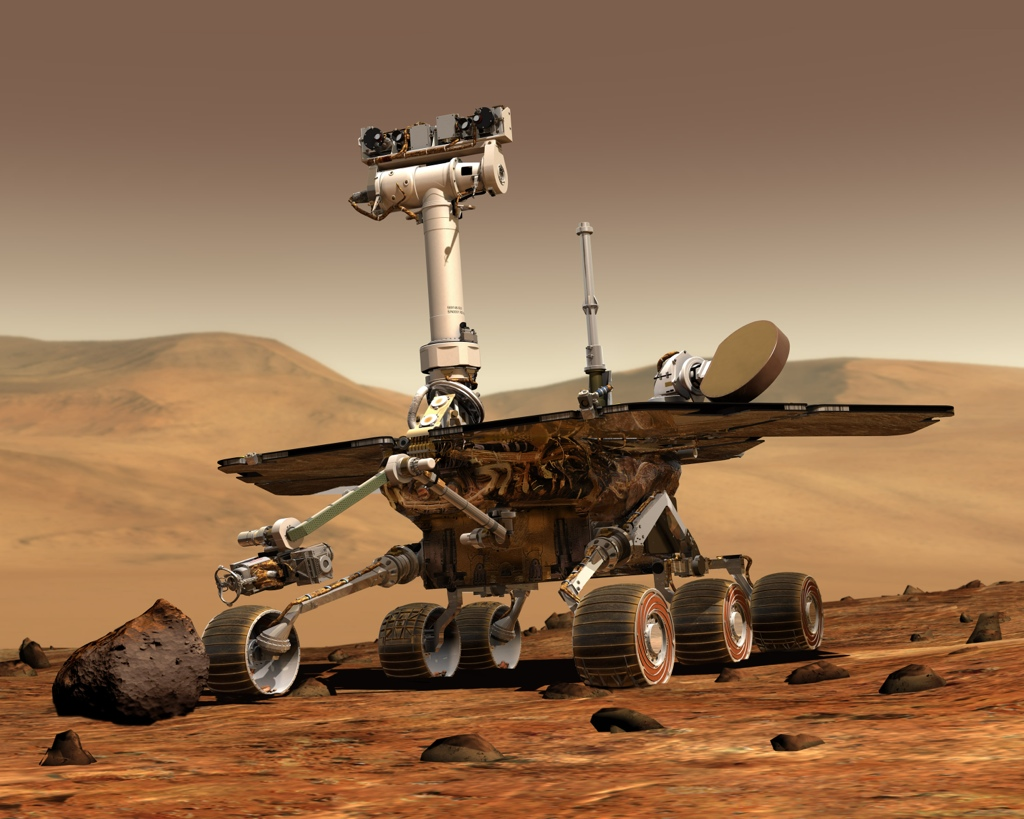
\includegraphics[width=6cm]{kapitel3/nasa_rover}
  \caption{Ein Nasa Rover}
  \label{Kap2:NasaRover}
\end{figure}


Man kann sich auch selber ein Makro für das Einfügen von Bildern schreiben:

\bild{kapitel3/modell_point_to_point}{6cm}{Point to Point}

\begin{sidewaysfigure}
 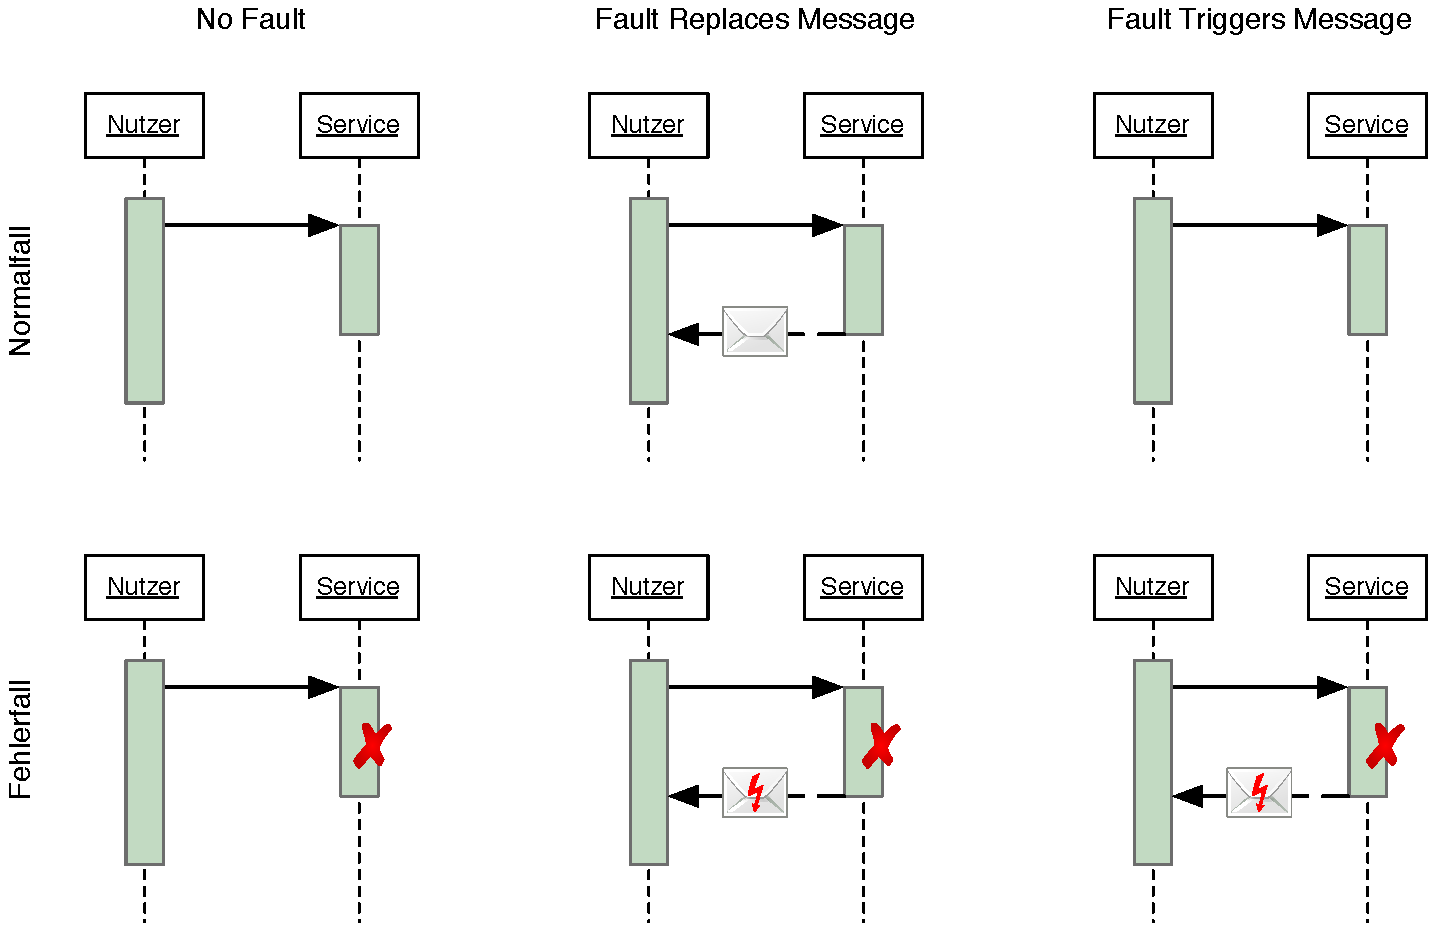
\includegraphics[width=22cm]{kapitel3/ws-wsdl20-fehler}
  \caption{Sehr große Grafiken kann man drehen, damit sie auf die Seite passen}
  \label{Kap2:wsdl-fehler}
\end{sidewaysfigure}


\clearpage % Alle Bilder, die bisher kamen ausgeben

\section{Formelsatz}

Eine Formel gefällig? Mitten im Text $a_2 = \sqrt{x^3}$ oder als eigener Absatz (siehe Formel~\ref{Formel}):

\begin{equation}
\begin{bmatrix}         
   1 &  4 &  2 \\
   4 &  0 & -3 
\end{bmatrix}        
        \cdot
\begin{bmatrix}                
   1 &  1 &  0 \\
  -2 &  3 &  5 \\
   0 &  1 &  4 
\end{bmatrix}        
       {=} 
\begin{bmatrix}               
  -7 &  15 &  28 \\
   4 &   1 & -12 
\end{bmatrix}
\label{Formel}
\end{equation}


\section{Sourcecode}

Man kann mit Latex auch ganz toll Sourcecode in den Text aufnehmen.

\subsection{Aus einer Datei}

\lstinputlisting[firstline=2,language=Java,caption={Crypter-Interface},label=lst:CrypterInterface]{\srcloc/Crypter.java}


\subsection{Inline}

\begin{lstlisting}[language=Java,caption=Methode checkKey()]
    /**
     * Testet den Schlüssel auf Korrektheit: Er muss mindestens die Länge 1
     * haben und darf nur Zeichen von A-Z enthalten.
     *
     * @param key zu testender Schlüssel
     * @throws CrypterException wenn der Schlüssel nicht OK ist.
     */
    protected void checkKey(Key key) throws CrypterException {

        // Passt die Länge?
        if (key.getKey().length == 0) {
            throw new CrypterException("Der Schlüssel muss mindestens " +
                    "ein Zeichen lang sein");
        }

        checkCharacters(key.getKey(), ALPHABET);
    }
\end{lstlisting}

 % Externe Datei einbinden
\chapter{Introduction}
To start this thesis a motivation for this scientific work is given. Then, the required knowledge is presented. After the presentation of the basic knowledge the objective of this bachelor thesis is displayed. To close this chapter an outline of this paper is given in the last section.

\section{Motivation}
One of several requirements regarding complex life is cell adhesion. If cells do not stick to each other the only living things would be cells. 
In humans and animals, organs and epithels are made of several cells and several layers of cells. This is also the case for the urothelium, which is an epithelium, i.e. a membranous tissue which consists of one or several layers. For the urothelium it is necessary that the cells stick to each other. Otherwise the functions of the urothelium could not be executed and also it would not be able to grow.

There are two types of tumors. One is the benign and the other one is the malignant tumor \cite{Poplawski2009}. The benign tumor is self limited. Thus, it does not invade surrounding tissues nor does it spread into other body parts \cite{Poplawski2009}. The malignant tumor on the other hand is not limited in its growth and is able to invade other body parts \cite{Poplawski2009}. 

Since bladder cancer is one of the most common cancer types among men it is important to understand how and why the cancer is able to grow. \newline
Bladder cancer starts to grow in the urothelium. With its growth and spread, the structure of cells sticking together changes. In this case, the urothelium is no longer able to completely perform its tasks. In order to understand the urothelium, how and when bladder cancer appears, it is necessary to observe the epithel.

To understand the functionalities of organs and epithels, in general organisms, observations are essential. For the urothelium this is already done as there are several in vitro experiments about the methodology of the urothelium \cite{WRCross2005, PuneetKhandelwal2009}. After an observation of an epithel or organ is complete, researches are able to predict how the observed organism will react in different situations. To verify these predictions a simulation is necessary. A simulation is an abstract illustration of the reality, but it can also be used to change reality in a for the research specific way, to get more knowledge of the epithel, or an organism in general.

A simulation should always be as simple as possible but not too simple. Otherwise the simulation does not represent the reality. 
There are several programs with different algorithms for cell simulation. A popular approach is the \ac{GGH} model. This model is popular because it is easy to describe how cells interact with each other and it is possible to define constraints for the volume and surface of each cell. \newline
The program \ac{CC3D} is a simulation program, which uses the \ac{GGH} algorithm in its simulation. In the moduro project \ac{CC3D} is used, and with the program the \ac{GGH} algorithm is used.

The target of the moduro project is to predict under which circumstances bladder cancer occurs and when it is able to grow. Therefore, 16 different morphogenesis models of the urothelium were created. An overview of these models is displayed in table \ref{tbl:16Models} at page \pageref{tbl:16Models}. So far, all 16 models were simulated in 2D for a timespan of 720 days. The results reveal that some of the models are more realistic than others.

A 2D simulation of the urothelium might not give as many aspects as a 3D simulation could do, because a cell is a three dimensional organism. Thus, the aim of this bachelor thesis is to create a 3D simulation of these 16 different models. With this 3D simulation it is hoped to receive new insights into the urothelium and how bladder cancer occurs.

\section{Background}
\subsection{Biology of the Urothelium}
Bladder cancer is the fourth most common cancer type in men according to everydayhealth.com \cite{EveryDayHealth.com}, every 36st out of 100.000 men gets it. Bladder cancer usually starts with some cells in the bladder growing uncontrolled. From these cells the tumor can spread further into surrounding areas \cite{Cancer.org}. The most common bladder cancer type is urothelial carcinoma \cite{Cancer.org}.

The bladder is located in the lower urinary tract and consists of several parts. The urothelium is one part of it and coats the bladder \cite{Lazzeri2006}. More specifically, it covers the bladder from the renal pelvis to the proximal urethra \cite{Yamany2014, Birder2005}.

Two important tasks of the bladder are the storage and release of urine. To do so the bladder will extend, during the storage, and then shrink again \cite{Karl-ErikAndersson2004}. One task of the urothelium is to form a distensible barrier \cite{Apodaca2004, Lazzeri2006, PuneetKhandelwal2009, Lewis2000, WRCross2005}, which prevents unregulated exchange of ions, solutes, and toxic metabolites between the bladder and the blood \cite{Apodaca2004, Lazzeri2006, PuneetKhandelwal2009, Lewis2000}. The urothelium ensures its barrier function through enlargement and downsizing of its size. This is done by the largest cells of the urothelium, the umbrella cells, also called superficial cells. Since the umbrella cells are in direct contact with the bladder it is their task to change size and form during the growth and shrink process of the bladder. Birder \cite{Birder2005} described the urothelium as “… a responsive structure capable of detecting physiological and chemical stimuli and releasing a number of signaling mole-cules.”. Another task of the urothelium is to control the movement and passage of macromolecules, ions, water, toxic metabolites and solutes \cite{Apodaca2004, PuneetKhandelwal2009}. If the urothelium is damaged, it rapidly generates new cells, to ensure full functionality \cite{Apodaca2004, Yamany2014, PuneetKhandelwal2009}.

To receive a better overview of the different cell types, they are explained in the following paragraph. In figure \ref{img:physiology_urothelium} a simplified illustration of the urothelium with its different cell types and cell layers is provided. \newline
The umbrella cells are connected directly with the bladder and have an average diameter of 25 up to \SI{250}{\micro\metre} \cite{Yamany2014, PuneetKhandelwal2009}. 

Below these cells the intermediate cells are located, with an average diameter of 10 up to \SI{20}{\micro\metre} \cite{Yamany2014, PuneetKhandelwal2009}. There are at least three and up to five layers of the intermediate cells \cite{PuneetKhandelwal2009}. 

The smallest and the most common cells in the urothelium are the basal and stem cells. Those cells have a diameter of up to \SI{10}{\micro\metre} \cite{Lazzeri2006, PuneetKhandelwal2009}. 

The urothelium consists of several layers. In the first layer, there are the basal and stem cells. Above them, there are several layers of intermediate cells. On top of the epithelium is one layer of umbrella cells.


\begin{figure}[th]
	\center
	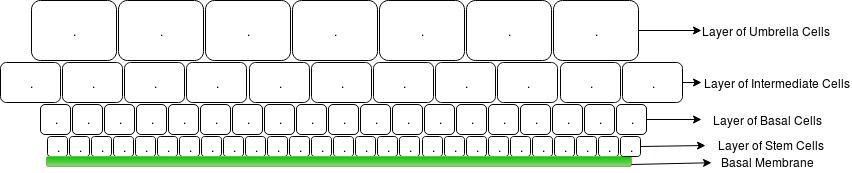
\includegraphics[scale=0.3]{figures/Urothelium.png}
	\caption[A simplified illustration of the urothelium]{A simplified illustration of the urothelium. At the very bottom is the basal membrane. Above the membrane the stem and basal cells are displayed. The blue cells represent the stem cells, the red cells display the basal cells. Above the layer out of these two cell types, the urothelium contains several layers of intermediate cells. At the top of the urothelium is a layer of umbrella cells.}
	\label{img:physiology_urothelium}
\end{figure}

\subsection{CompuCell3D}
\ac{CC3D} is an open-source program, which provides a simulation environment for multi- or single-cell-based modeling of tissues, organs and organisms \cite{CC3D.org}. To do so, \ac{CC3D} uses the \ac{GGH} model in its simulation. 
CC3D provides the possibility to create programs for the simulation, e.g. cell growth, mitosis, apoptosis or necrosis scripts, in Python, C++ or in CC3DML, which is their own Markup Language. With such programs CC3D allows the user to modify the behavior of the simulation for a specific purpose.
CC3D uses the \ac{GGH} approach, which is explained in the next section. It allows the user to choose between two cell-lattice types, i.e. a presentation of the pixels or voxels, i.e. a pixel with three dimensions, of a cell at a specific position in the simulation field. By default, it uses a square-lattice of single pixels for each dimension, an example therefore is displayed in figure \ref{img:2DSquareLattice}. \ac{CC3D} provides the possibility to use a hexagonal-lattice, where the pixels are hexagons in two dimensions, or rhombic dodecahedrons in three dimensions.
The core of a \ac{GGH} simulation is the effective energy \cite{MaciejH.Swat2017}, \ac{CC3D} tries to minimize this effective energy every \ac{MCS}, i.e. a calculation step in the simulation. The basic form for the effective energy is:

\begin{equation}
\mathcal{H}_{boundary} = \sum_{\vec{i},\vec{j}}^{ }{J(\tau(\sigma(\vec{i})),(\tau(\sigma(\vec{j})))(1-\delta(\sigma(\vec{i}),(\sigma(\vec{j})))}
\end{equation}
This equation is a part of the equation of the \ac{GGH} model. This model is explained in the next section. It is possible to extend this form in two ways. Either a volume or a surface constraints for each cell can be added. 
During each \ac{MCS} an index-copy attempt takes place \cite{MaciejH.Swat2017}. In this index-copy attempt a pixel is selected, and it is tried to overwrite a randomly chosen pixel, next to the current pixel. It succeeds and takes place if this index copy attempt decreases the effective energy \cite{MaciejH.Swat2017}. Each \ac{MCS} \ac{CC3D} tries to minimize the effective energy with index copy attempts. 

\begin{figure}[th]
	\center
	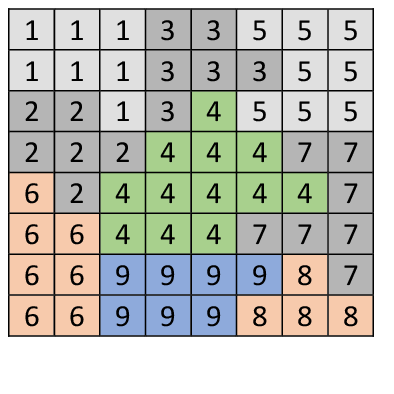
\includegraphics[scale=0.4]{figures/2DSquareLattice.png}
	\caption[A two dimensional square lattice]{A square lattice in 2D. The same digits represent one cell $(\sigma(\vec{i}))$, whereas the different colors represent different cell types $\tau(\sigma)$.}
	\label{img:2DSquareLattice}
\end{figure}

\subsection{Glazier Graner Hogeweg Model} \label{subsec:Intro_GGH}
Glazier and Graner developed several formulas and models which are presented in this subsection with focus on the \ac{CPM} and \ac{GGH} model.\newline
The \ac{GGH} model is widely used in biological simulations, since it provides a good flexibility, extensibility and usability \cite{Glazier2007}. 
Glazier and Graner \cite{Glazier2007} developed the \ac{EPM} as an extension of the large-q Potts model, which itself is an extension of the Ising Model. Nowadays, this model is called \ac{CPM} \cite{Glazier2007, Graner1992, Glazier1993}. Glazier and Graner extended the \ac{CPM} in a way that also volume constraints are considered for the Hamiltonian, i.e. the effective energy, as it is displayed in the following equation:

\begin{equation}\label{eq:H_CPM}
\begin{split}
\mathcal{H}_{CPM} & = \sum_{\vec{i},\vec{j}}^{ }J(\tau(\sigma(\vec{i})),(\tau(\sigma(\vec{j})))(1-\delta(\sigma(\vec{i}),(\sigma(\vec{j}))) \\
		 & + \sum_{\sigma}^{}{\lambda_{vol}((\tau)v(\sigma)-V_{target}(\tau(\sigma)))^2}
\end{split}
\end{equation}
The Hamiltonian of equation \ref{eq:H_CPM} describes the effective energy for the extension of the \ac{CPM} model. The first sum describes $J$ of all cells, the adhesion energy between different cells. Therefore, every cell has a specific cell type $\tau(\sigma)$ \cite{Glazier1993, Graner1992}. Each cell is placed onto a lattice with a spin $(\sigma(\vec{i}))$ for every given dimension \cite{Graner1992, Glazier2007}. The adhesion energy between cells is only considered if the Kronecker delta is 0. Thus, the adhesion energy between cells is considered if $\delta(\sigma, \sigma') = 0$ \cite{Glazier1993, Graner1992, Stott1999, Glazier2007, Chen2007, Cickovski2005}. \newline
With the second sum over all cells the volume of each cell is now considered within the effective energy. The user is now able to set a target volume $V_{target}(\tau(\sigma))$ for each cell and a multiplier $\lambda_{vol}$ for the deviation between the current volume $(\tau)v(\sigma)$ and the target volume. During the simulation this deviation is tried to be kept as small as possible for every cell in order to keep the effective energy as small as possible.

Together with Hogeweg Glazier and Graner further developed the created extension of the \ac{CPM}. The further developed model is called \ac{GGH} model. The main extension is that the user is now able to add surface area constraints \cite{Graner1992, Glazier1993, Glazier2007} as well as to use a negative boundary energy \cite{Glazier2007}. With the surface constraint the equation for the effective energy of the \ac{GGH} model is:

\begin{equation}\label{eq:H_GGH}
\begin{split}
\mathcal{H}_{GGH} & = \sum_{\vec{i},\vec{j}}^{ }J(\tau(\sigma(\vec{i})),(\tau(\sigma(\vec{j})))(1-\delta(\sigma(\vec{i}),(\sigma(\vec{j}))) \\
		 & + \sum_{\sigma}^{}{\lambda_{vol}(\tau)v(\sigma)-V_{target}(\tau(\sigma)))^2} \\
		 & + \sum_{\sigma}^{}{\lambda_{sur}(\tau)s(\sigma)-S_{target}(\tau(\sigma)))^2}
\end{split}
\end{equation}
In addition to the Hamiltonian of equation \ref{eq:H_CPM} is the surface constraint. It has the same principle as the volume constraint. Thus, the user is able to define a target surface $S_{target}(\tau(\sigma))$ for each cell and a multiplier $\lambda_{sur}$ for the deviation between the target and the actual surface $(\tau)s(\sigma)$ of each cell. Since the volume and surface constraint are included in the effective energy, it should be possible to use these two parts of the effective energy to shape the cells.


Beside the surface constraint the new model allows the user to model (a): cell growth and proliferation (b): mitosis, i.e. cell division (c): fields, forces and diffusion and (d): chemotaxis and haptotaxis \cite{Glazier2007}. \newline
Glazier et. al. describe their models as: 
\begin{quote}
"GGH models define biological structure consisting of the configuration of a set of \textit{generalized cells}, each represented on a \textit{cell lattice} as a domain of lattice sites sharing the same cell index [...], a set of \textit{internal cell states} for each cell [...], and a set of \textit{auxiliary fields} ...” \cite{Glazier2007}.
\end{quote}

“Initial conditions emulating a particular biological configuration rather than random initial conditions.” \cite{Glazier2007} brings the advantage that the \ac{GGH} model now has biologically motivated properties instead of physically motivated properties \cite{Glazier2007}.



\section{Objective}
The aim of this bachelor thesis is to create a 3D morphogenesis simulation of the urothelium using \ac{CC3D}.  The task is to modify the current application, of the 2D simulation, in a way that this program can be used for a 3D simulation, because the simulation models and the program for a 2D simulation are given and the simulation is done by \ac{CC3D}. \newline
The required changes are all in the program, because the models of the 2D simulation should be also used for the 3D simulation.
Therefore, some parts of the program have to be modified whereas other parts have to be developed. It is possible to try to let the cell have a different shape than in the 2D simulation, because a third dimension will be added to the simulation.
The result of this bachelor thesis will be presented with an analysis of a 3D simulation. A model therefore is selected out of the models which were created earlier in the project. These models are explained in section \ref{sec:Models} at page \pageref{sec:Models}.


\section{Outline}
Chapter 'State of the Art' provides the status at which the project was at the beginning of this bachelor thesis. Once the basic knowledge and the 'State of the Art' are explained, the modifications in the program during this journey are revealed in chapter 'Methods'. Then, in chapter 'Results' the outcome of this thesis is presented. After the results are presented, they are discussed of different perspectives in chapter 'Discussion'. In chapter 'Future Work' ideas for the future of the project are presented and to round up this paper a conclusion is provided in chapter 'Conclusion'.
\chapter{State of the Art}
%What was given to me
In this chapter all information about the current project are revealed. At the beginning the properties of the project are explained and later in this chapter the simulation program is presented. The sections \ref{sec:Adhesion} to \ref{sec:3D} are explained based on the program of the project, wheras the other sections are presented based on previous work of the project.

\section{Moduro}
In the project moduro stands for 'Modeling of the Urothelium with the \ac{GGH} approach'. \newline
The department of Medical Informatics at the University of Applied Sciences Mannheim and the Clinic of Urology in cooperation with the Medical Faculty Mannheim at the University of Heidelberg participate in this project. The aim is to predict how and when bladder cancer arises.

The current moduro project has a stable 2D simulation of 16 different models using \ac{CC3D}. The simulations are performed by \ac{CC3D}. During the simulation statistics about the current simulation are written in text files and can be read out by the moduro toolbox. \newline
The project consists  of a program and several models, both are written in python. The models include properties of cell behavior. Therefore, the adhesion energy between cells and the possibilities of the new cell types after mitosis is defined in the different models. The application modifies the cell behavior, for instace it checks when a mitosis takes place and how fast the cell will growth.

\section{Display and Simulation of the Urothelium}
%wie wird es dargestellt 
In the 2D simulation, the urothel is simulated with a size of \SI{500}{\micro\metre} for the x-axis and \SI{150}{\micro\metre} for the y-axis. Because, the voxel density is $0.8$, the size of the urothelium is represented with 400 pixels at the x-axis and 120 pixels at the y-axis. The voxel denstity describes how many pixels are used to display \SI{1}{\micro\metre}. \ac{CC3D} allows the user to use any simulation size, as long as the required hardware is able to handle the simulation. \newline
It is possible to use \ac{CC3D} on several cores of the CPU. In the project one core for a simulation is used, because otherwise \ac{CC3D} splits the simulation field into different grids. As a result race conditions can occur at the edges of these grids \cite{MaciejH.Swat2017}. This means it is possible that a cell is in both grids. Thus, one half is in one grid and the other half is in another grid. During the simulation both grids calculate the volume of the cell and both apply the new volume of their calculation but it is not checked which result has to be used. Therefore, in order to reduce wrong results, it is necessary to avoid race conditions. \newline 
The 2D simulations of the urothelium covered 720 days. In the simulations one day is split up into 500 \ac{MCS}. Therefore, the simulation covers 360000 \ac{MCS}. The simulation duration can be set in the program. Thus, the user defines how many \ac{MCS} simulate one day and how long the simulation runs. At the first calculation step, \ac{MCS} 0, the simulation is initialized, i.e. the cells are drawn and placed on the basal membrane. An illustration of an initial simulation is displayed in figure \ref{img:2DSimulationInitialState}. Since morphogenesis is simulated, the urothelium is proposed to growth and to proliferate in the given area. An illustration therefor is presented in figure \ref{img:2DSimulation33Days}.

\begin{figure}
	\center
	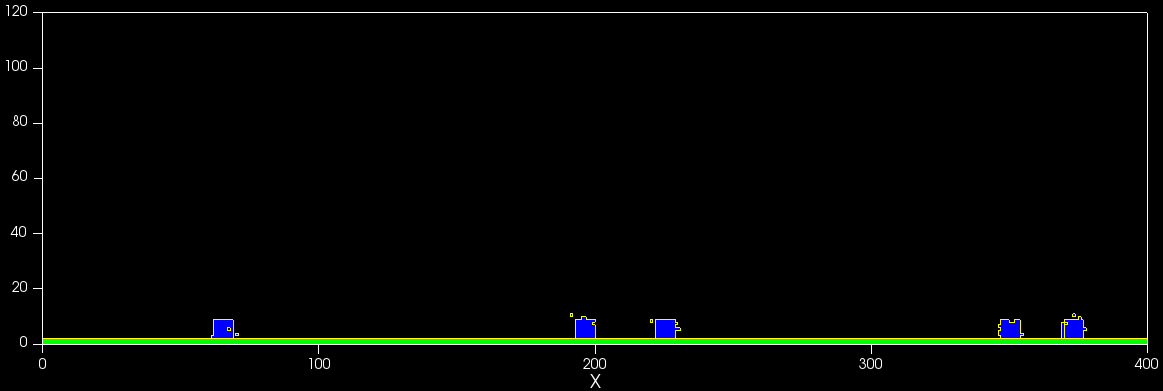
\includegraphics[scale=0.35]{figures/2DSimulation-InitialState.png}
	\caption{Initial state of a 2D simulation of the model SPA/BPCD/IPCD}
	\label{img:2DSimulationInitialState}
\end{figure}

\begin{figure}
	\center
	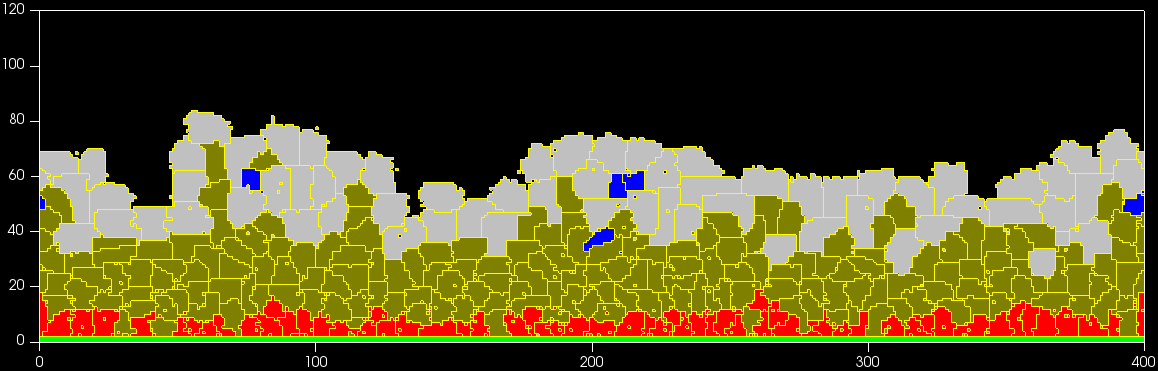
\includegraphics[scale=0.35]{figures/2DSimulation-33Days.png}
	\caption{2D Simulation of the model SPA/BPCD/IPCD after 33 days}
	\label{img:2DSimulation33Days}
\end{figure}

\section{Moduro Toolbox}
The moduro toolbox is a software tool, which is able to visualize data in order to evaluate a simulation. \newline
Every 12 hours the simulation is checked for its reality. This is done with the fitness functions of section \ref{sec:fitnessFunctions}. The results of these calculations are written in several text files, in a by \ac{CC3D} created directory of the simulation. Moreover, the amount of cells of the different cell types and the overall amount of cells is saved as well. The moduro toolbox is able to read out the data of the text files and then visualize these. This visualization is done with charts and with a table. \newline
\ac{CC3D} saves some screenshots, of the simulation field, during the simulation. With these screenshots the moduro toolbox is able to create a video out of these screenshots. To create the video an extra program has to be installed which the toolbox would use.

\section{Models}\label{sec:Models}
The 2D simulation of the urothel provides 16 different models. These models differ mostly in which cell types after the mitosis are created. The project divides the models into two domains, one has the identifier 'SSD' and means that every time a stem cell divides there will be one stem and one basal cell. The second domain is called 'SPA'. In the second domain the stem cell has a probability of 90\% that it will be one stem and one basal cells after mitosis. There is also the chance with a probability of 5\% that after mitosis of a stem cell there are two stem cells or two basal cells. \newline
For the mitosis of basal cells there are 4 different models. The mitosis model 'BSD' describes that each basal cell which undergoes mitosis will create one basal and one intermediate cell. The model 'BPA' describes that there is a 5\% chance that the basal cell will become two basal or two intermediate cells. There is a 90\% probability that the cell become one basal and one intermediate cell. The model 'BPCD', describes that always a basal cell becomes two basal cells during mitosis and if the basal cell is not on the basal membrane it transform into an intermediate cell. The model 'BCD' has the behavior that a basal cell immediately transforms into an intermediate cell if it is not at the basal membrane.\newline
There are two different models how intermediate cells split. One is the 'IPCD', therefor in mitosis an intermediate cell becomes two intermediate cells during. Each \ac{MCS} it is checked if there is a cell around the intermediate cell. If this is not the case it is transformed into an umbrella cell. The second model is the 'ICD'. In this one, only transformation of the intermediate cells into the umbrella cells happens if the intermediate cell is not enclosed by other cells. \newline
With these mitosis concepts there are 16 different models in the project. These models were created by an earlier version of the project \cite{Torelli2017} and are displayed in table \ref{tbl:16Models} at page \pageref{tbl:16Models}.


\begin{table}
\begin{centering}
\par\end{centering}
\begin{centering}
\begin{tabularx}{\textwidth}{|c|c|Xc|}
\hline 
Type & ID & Description & Model\tabularnewline
\hline 
\hline 
\multirow{2}{0.02\textwidth}{\begin{turn}{90}
Stem cells
\end{turn}} & SSD & Stem cell-like division & \begin{tikzpicture}[]
\node[SType] {S} [grow=right]
	child {node [SType]  {S}
	}
	child {node [BType]  {B}
	};
\end{tikzpicture}\tabularnewline
\cline{2-4} 
 & SPA & Stem cell population asymmetry & \begin{tikzpicture}[]
\node[SType] {S} [grow=right]
	child {node [SType]  {S}
	}
	child {node [SType]  {S}
	};
\node at (0.5,-1) {$p_s=0.05$};
\node[SType] at (2,0) {S} [grow=right]
	child {node [SType]  {S}
	}
	child {node [BType]  {B}
	};    
\node at (2.5,-1) {$p_a=0.90$};    
\node[SType] at (4,0) {S} [grow=right]
	child {node [BType]  {B}
	}
	child {node [BType]  {B}
	};    
\node at (4.5,-1) {$p_s=0.05$};        
\end{tikzpicture}
\tabularnewline
\hline 
\multirow{4}{0.02\textwidth}{\begin{turn}{90}
Basal cells\ \ \ \ \ \ \ \ \ \ \ \ \ \ \ \ \ \ \ \
\end{turn}} & BSD & Stem cell-like division in basal cell & 
\begin{tikzpicture}[]
\node[BType] {B} [grow=right]
	child {node [IType]  {I}
	}
	child {node [BType]  {B}
	};
\end{tikzpicture}
\tabularnewline
\cline{2-4} 
 & BPA & Basal cell population asymmetry & \begin{tikzpicture}[]
\node[BType] {B} [grow=right]
	child {node [BType]  {B}
	}
	child {node [BType]  {B}
	};
\node at (0.5,-1) {$p_s=0.05$};
\node[BType] at (2,0) {B} [grow=right]
	child {node [BType]  {B}
	}
	child {node [IType]  {I}
	};    
\node at (2.5,-1) {$p_a=0.90$};    
\node[BType] at (4,0) {B} [grow=right]
	child {node [IType]  {I}
	}
	child {node [IType]  {I}
	};    
\node at (4.5,-1) {$p_s=0.05$};        
\end{tikzpicture}\tabularnewline
\cline{2-4} 
 & BPCD & Proliferation and contact differentiation of basal cells & \begin{tikzpicture}[]
\node[BType] {B} [grow=right]
	child {node [BType]  {B}
	}
	child {node [BType]  {B}
	};
\end{tikzpicture} \hspace{1em} and \hspace{1em}
\begin{tikzpicture}[]
\node[BType] {B} [grow=right]
	child[dashed] {node [IType] {I} edge from parent node[above=0.4cm] {$\neg$ BM}
	};
\end{tikzpicture}\tabularnewline
\cline{2-4} 
 & BCD & Only contact differentiation of basal cells & 
\begin{tikzpicture}[]
\node[BType] {B} [grow=right]
	child[dashed] {node [IType] {I} edge from parent node[above=0.4cm] {$\neg$ BM}
	};
\end{tikzpicture}\tabularnewline
\hline 
\multirow{2}{0.02\textwidth}{\begin{turn}{90}
Intermediate cells
\end{turn}} & IPCD & Proliferation and contact differentiation of intermediate cells & \begin{tikzpicture}[]
\node[IType] {I} [grow=right]
	child {node [IType]  {I}
	}
	child {node [IType]  {I}
	};
\end{tikzpicture} \hspace{1em} and \hspace{1em}
\begin{tikzpicture}[]
\node[IType] {I} [grow=right]
	child[dashed] {node [UType] {U} edge from parent node[above=0.4cm] {M}
	};
\end{tikzpicture}
\tabularnewline
\cline{2-4} 
 & ICD & Only contact differentiation of intermediate cells & 
\begin{tikzpicture}[]
\node[IType] {I} [grow=right]
	child[dashed] {node [UType] {U} edge from parent node[above=0.4cm] {M}
	};
\end{tikzpicture}
\tabularnewline
\hline 
\end{tabularx}
\par\end{centering}
\caption{\label{tbl:16Models}16 different models derived in the project as there are different ways of proliferation and mitosis are simulated for the different cell types.}
\end{table}




\section{Adhesion}\label{sec:Adhesion}
During morphogenesis the cells not only growth, they also sort themselves. For cell sorting there have to be different adhesion values, i.e. how strong two different cells are holding on each other. In the project this is done with a matrix, which every of the 16 model has. Such a matrix was created in an earlier version of the project \cite{Torelli2017} and is displayed in table \ref{tbl:AdhesionMatrix} at page \pageref{tbl:AdhesionMatrix}.

\begin{table}
\begin{centering}
\begin{tabular}{|c|c||c|c|c|c|c|c|}
\hline 
\multicolumn{2}{|c||}{Types} & M & BM & \celltypeS & \celltypeB & \celltypeI & \celltypeU \tabularnewline
\hline 
\hline 
Medium & M & 0 & 14 & 14 & 14 & 14 & 4\tabularnewline
\hline 
Basal membrane & BM &  & -1 & 1 & 3 & 12 & 12\tabularnewline
\hline 
Stem cell & \celltypeS &  &  & 6 & 4 & 8 & 14\tabularnewline
\hline 
Basal cell & \celltypeB &  &  &  & 5 & 8 & 12\tabularnewline
\hline 
Intermediate cell & \celltypeI &  &  &  &  & 6 & 4\tabularnewline
\hline 
Umbrella cell & \celltypeU &  &  &  &  &  & 2\tabularnewline
\hline 
\end{tabular}
\par\end{centering}
\caption{\label{tbl:AdhesionMatrix}Adhesion matrix for a model in the simulation. Smaller values refer to more adhesion and higher values mean less adhesion. The cell type M is the medium cell type, it is by \ac{CC3D} a specific cell type which is every in the available space in the simulation, and BM is the basal membrane.}
\end{table}


\section{Cell properties}
In the project the physiology constraints of a cell are included. In an earlier version of the project these were evidenced \cite{Torelli2017} and are displayed in table \ref{tbl:CellConstraints} at page \pageref{tbl:CellConstraints}. In the program these constraints are converted into pixels and then applied. \newline
In the simulation every cell has several attributes. Moreover, each cell has an cell dictionary, in which additional attributes are stored. The properties regarding the cell type are likely what every cell in general has, e.g. a min- max diameter, a min- max volume, growth in \SI{}{\micro\metre} per day or the time until apoptosis, i.e. cell death. \newline
The attributes in the cell dictionary are mainly used for decision making. Some values are the current and expected live time, a flag for necrosis and if a cell is inhibited, i.e. enclosed by other cells. \newline



\begin{table}
\begin{centering}
\begin{tabular}{|cc|c|c|c|c|c|c|}
\hline 
Cell type & & $V_{min}$ & $d_{min}$ & $V_{max}$ & $d_{max}$ & Volume & Surface\tabularnewline
\hline 
\hline 
Stem & \celltypeS & 268 & 8 & 523 & 10 & perfect & average\tabularnewline
\hline 
Basal & \celltypeB & 381 & 9 & 523 & 10 & important & average\tabularnewline
\hline 
Intermediate & \celltypeI & 905 & 12 & 1767 & 15 & important & poor\tabularnewline
\hline 
Umbrella & \celltypeU & 1767 & 15 & 3591 & 19 & important & poor\tabularnewline
\hline 
\end{tabular}
\par\end{centering}
\caption{\label{tbl:CellConstraints}Constraints of a cell. Volumes $V$ in $\mu$m$^{3}$, diameters $d$ in $\mu$m. The 'Volume' and 'Surface' column describe how the $\lambda_{vol}$ and the $\lambda_{sur}$ should be set for each cell type.}
\end{table}





\section{Events in the simulation}
In the simulation program there are several events modeled. These events can occur every calculation step or at a specific \ac{MCS} in the simulation. \newline
The events which are performed every \ac{MCS}, except for \ac{MCS} 0 and every \ac{MCS} of factor 250, are a) cell growth and b) the check for mitosis c) cell death d) cell transformation and e) cell mutation. The event which occurs every 12 hours, every 250 \ac{MCS}, is f) urination. These events are presented in detail in the following subsections.

\subsection{Cell Growth}
In the project the maximum possible growth of a cell is calculated and applied. This calculation is used for the relation volume and target volume as well as for the relation volume, surface and target surface. Because, the volume and the surface of a cell is calculated by \ac{CC3D} and can only be read out, the target volume and target surface are calculated in the program and set.

\subsection{Mitosis}
The verification if a cell divides or growth further is done in every simulation step, except for these with a factor of 250. Therefore, it is possible to define a very specific calculation step at which a cell divides, as there a 500 \ac{MCS} per day. In order that a cell divides it grows over its maximal size before it divides.
The cells which are able to grow and as a result divide are a) stem cells b) basal cells and c) intermediate cells. The umbrella cells grow as well, but they do not split.

\subsection{Necrosis}
If a cell dies, necrosis takes place. In the program a flag in the cell dictionary is set. Every calculation step, except for the \ac{MCS} of factor 250, the program checks if a cell dies or not. If so, the cell will shrink and as a result disappear.

\subsection{Mutation}
After 2 days, 1000\ac{MCS}, it is possible that a cell mutates, i.e. it becomes malignant. We simulate the possibility for cells to mutate after 2 days, because otherwise there would not be much cells around the mutated cell. Each cell type has its own probability to become malignant. In the current simulation it is not considered that cells mutate since the probability for each cell type to mutate is 0\%. \newline
If a cell mutates, there is also the flag for necrosis set. Thus, the cell shrinks and disappears.

\subsection{Transformation}
A transformation can take place if a basal cell divides and at least one intermediate cell is created. If the intermediate cell is not enclosed by other cells, it immediately will be transformed to an umbrella cell.

\subsection{Urination}
Every 12 hours, every 500 \ac{MCS}, a urination takes place. The first urination event takes place at \ac{MCS} 375. This is simulated in a way that randomly 2\% of the cells in direct contact with the bladder are washed out. In the program a flag for necrosis is set and the cells will disappear because of the necrosis event.



\section{Fitness functions}\label{sec:fitnessFunctions}
In order to validate the simulated models, there are several functionalities which check if the model is realistic or not. These functions, i.e. part of a program, check every 12 hours, every 250 \ac{MCS}, if the model is realistic or not. The result of these fitness functions is written into several files, and can be read out by the moduro toolbox.

\subsection{Arrangement fitness function}
The arrangement fitness function ensures that the strata of the simulated urothelium has the correct order \cite{Torelli2017}, i.e. that the first layer on the basal membrane consists only of stem and basal cells \cite{REFS}, the next three to five layers consists only of intermediate cells \cite{REFS} and that there is one layer of umbrella cells \cite{REFS}.

\begin{equation}\label{eq:LIB}
lib = \dfrac{L - lib}{L}
\end{equation}
\begin{equation}\label{eq:FitnessArrangement} 
f_{a} = 1 - \dfrac{((1-L_{B})+(1-L_{U})+lib+(1-L_{O})}{4}
\end{equation}
In equation \ref{eq:LIB} $L$ refers to the amount of layers in the urothelium. $lib$ describe the amount of layers between the stem and basal cell layer and the umbrella cell layer at the top of the urotehlium, which include not only intermediate cells. Thus, if the layers between the first and last layer consist only of intermediate cells, the equation \ref{eq:LIB} has the result 0.\newline
In equation \ref{eq:FitnessArrangement} $L_{B}$ and $L_{U}$ are boolean values, i.e. they have the value 0 or 1 and represent a false or true value. They are 1 if the first layer of cells consists only of basal or stem cells and if the most upper layer consists only of umbrella cells, otherwise they will be 0.
$lib$ is calculated in equation \ref{eq:LIB}. $L_{O}$ presents the optimum amount of layers. It is 1, if the amount of layers in the simulated urothelium is between 3 and 7, otherwise it is 0. The result of equation \ref{eq:FitnessArrangement} is between 0 and 1, where 0 refers to no reality in the simulation and 1 refers to a perfect simulated urothelium. \newline

\subsection{Volume fitness function}
This function calculates the relative volume regarding the current volume of the different cell types in the urothel. The relative amount of the different cell types should be: stem and basal cell = 10\%, intermediate cells = 67\% and umbrella cells = 23\% considering an average thickness of \SI{85}{\micro\metre} \cite{Torelli2017}. Therefor the formula is:
\begin{equation}\label{eq:VolumeFitnessSpecific}
f_{V_{i}} = \dfrac{1}{4 (\dfrac{V_{Si}-V_{Ii}}{V_{Si}})^2 + 1}
\end{equation}
$V_{Si}$ and $V_{Ii}$ describes the \textit{should} and the actual \textit{is} volume of a specific cell type $i$ \cite{Torelli2017}.  This calculation is done three times. One time for the stem and basal cells, one time for the intermediate cells and one time for the umbrella cells. The results of the three calculations are then further used to determine the relative volume overall.
\begin{equation}\label{eq:VolumeFitnessOverall}
f_{V} = \dfrac{f_{V_{B}} + f_{V_{I}} + f_{V_{U}}}{3}
\end{equation}
In this equation $f_{V_{B}}$ refers to the realtive volume of the stem and basal cells, $f_{V_{I}}$ presents the relative volume of the intermediate cells and $f_{V_{U}}$ include the realtive volume of the umbrella cells. \newline
The result of all four calculations are written into a text file and can be read out by the moduro toolbox later.

\subsection{Overall fitness function}
The overall fitness function calculates the total fitness out of the volume and the arrangement fitness function. Therefor the average of both functions is calculated \cite{Torelli2017}. This calculation is done by the moduro toolbox only. For every calculation step, the arrangement and volume fitness function are calculated the overall fitness is calculated. Therefor the formula is:

\begin{equation} 
f(t_{i}) = \dfrac{f_{V}(t_{i})+f_{a}(t_{i})}{2}
\end{equation}

$t_{i}$ describes a specific time point, in \ac{MCS}, at which this calculation is done. At the end of the simulation the average of the overall fitness function is calculated to determine the reality of this simulation. Therefor, the formula is:

\begin{equation} 
f = \dfrac{1}{e+1} + \sum_{i=0}^{e}{f(t_{i})}
\end{equation}
The result of the calculation is between 0 and 1. Where 0 describes no reality at all and 1 presents a perfect realistic simulated urothelium.


\section{3D functionalaties}\label{sec:3D}
The functionalaties of the program are able to be used in 3D. Whenever a part of the program is required to be used in 2D as well as in 3D, it is checked if the simulation field has a third dimension or not. Examples for such functionalities are the fitness functions of the section before or the decision how many stem cells are placed on the basal membrane, which is modified and explained in section \ref{sec:AmountStemCellsBasalMembrane}. \newline
Because so far only the 2D simulations were progressed, it is important to keep the functionalaties of the 2D simulation in the program. Doing so it is possible to switch between a 3D and a 2D simulation, as well as the benefits of both simulation types can be observed.
\chapter{Methods}
%just some stuff for the sphere in the cube graphic
\tikzset{
    MyPersp/.style={scale=1.8,x={(-0.8cm,-0.4cm)},y={(0.8cm,-0.4cm)},
    z={(0cm,1cm)}},
    MyPoints/.style={fill=white,draw=black,thick}
    }
    
This section has the purpose to give an overview over all changes in the project which occurred during this bachelor thesis. These changes include some small improvements of the application as well as how to draw a sphere cell. First minor changes are briefly described, deeper in this section the more effortful changes are explained. 

\section{Lambda multipliers}
In the project there were several places, where the multipliers $\lambda_{vol}$ and $\lambda_{sur}$ are calculated, but they are only set when a cell is initialized. The multiplier for the volume is set a second time in the necrosis event, if the program models that a cell dies. \newline
There are two additional multipliers, for the surface and volume constraints, saved in within each cell object. Since we are not using these values in the program and they do not influence or set the $\lambda_{vol}$ or $\lambda_{sur}$ which \ac{CC3D} uses, these two values are deleted. Moreover, in one place there were methods to calculate the lambda values. Since these methods are not used in the project and they had a multiplier itself to calculate the multiplier for the specific part of the effective energy, they are deleted as well. 

In the project the multipliers $\lambda_{vol}$ and $\lambda_{sur}$ are now set each time when a cell is initialized. A second time the multiplier $\lambda_{vol}$ is set, is if necrosis takes place. Because now the unnecessary methods and values for the multipliers values are removed, no confusion about which constraint values in the program are used will come up.

\section{Abstract methods}
In the program, in several classes there were methods, which are not used. These methods are not used in the class, in which they are written, due to polymorphism. They are used in classes, which inherit from the class where they are written. Polymorphism is a method out of \ac{OOP}. Another technique out of \ac{OOP} is the use of abstract classes and abstract methods. To explain polymorphism, abstract classes or abstract methods in detail, would take too much space out of this bachelor thesis. Thus, the change in the program is explained in the following.

In the project there a several classes which inherit from each other. In these classes there were the same methods implemented. Since it is not required that all classes have to have the same methods, these are redundant methods, as long as they do not differ in their functionality. For such methods it is possible to declare them as an abstract method. An abstract method contains only the method construct, but no functionality. Due to polymorphism the class in which such an abstract method is implemented is used to call this method. \newline
In python there is a library 'abc'. With this library it is possible to declare an abstract method. To do so every class with one or more abstract methods needs to initialize a special class variable. With this variable python is able to recognize that there are abstract methods included.

\begin{lstlisting}[language=Python, caption = The initialization of a class variable which is required by python in order to detect abstract methods and abstract classes.]
class ModelConfig(object):
    __metaclass__ = ABCMeta
\end{lstlisting}

The listing above displays how the class variable has to be initialized in order that abstract methods are recognized. If a class has at least one abstract method, it is an abstract class. In python abstract classes can include implemented methods as well as abstract methods.

\begin{lstlisting}[language=Python, caption = Declaration of an abstract method.]
    @abstractmethod
    def _createExecConfig(self):
        pass
\end{lstlisting}

The listing above is an example of an abstract method in python. Using abstract methods creates more structure and clarity within the project. Therefore, the abstract declarations in this project created a much better clarity of the structure of the project and of the methods, which were used in the classes.

\section{Calculation steps until urination}
To simulate the urination in the program it was checked if the current calculation step is larger than 250 and a factor of 125. Because every 250 \ac{MCS} the volume- and arrangement fitness functions are calculated and no other events in the simulation take place, the urination was simulated every 12 hours. The check if the current \ac{MCS} is a factor of 125 happens with the modulo operator. Thus, the current calculation step is divided by 125 and if the result, as a whole number, is 0 it is a factor. \newline
The check when the urination event takes place is modified. The urination event now takes place if the current calculation step is larger than 250 and if the current \ac{MCS} modulo 125 equals 1. Therefore, the urination event is used every 6 hours, at \ac{MCS} 376, 501, 626, 751, etc..

\section{Area of stem cells on the basal membrane}\label{sec:AmountStemCellsBasalMembrane}
In an earlier version of the project it was evidenced that around 12\% of the area of the basal membrane are required to be filled with stem cells in order to have an optimal proliferation during the morphogenesis of the cells \cite{Torelli2017}.
In the project the calculation of the amount of stem cells for two dimensions were correct but without an mathematical evidence. \newline
Since the y-axis is negligible in the calculation of an area, the calculation for two dimensions considers the x-axis and the calculation for three dimensions considers the x- and z-axis. Therefore, in two dimensions the area of the stem cells should be calculated by using the cell diameter. An illustration therefor is displayed in figure \ref{tikz:AreaIn2D}. For three dimensions it is possible to calculate the area of a circle with the formula $A = \pi \cdot r^{2}$, because a sphere in 2D is a circle, and use this calculation to further determine the amount of stem cells on the basal membrane. An example for the basal membrane and a stem cell in three dimensions is displayed in figure \ref{tikz:AreaIn3D}. 

\begin{figure}[h]
\begin{center}
\begin{tikzpicture}[scale=3]
%%draw the edges of the cube
\draw[black,thick] (-2,0) -- (2,0)node[anchor=north east]{$basal membrane$};
\draw[blue,thick] (-1,.01) -- (-0.5,.01)node[anchor=north]{$d_{cell}$};
\end{tikzpicture}
\caption{Considered area to spread the stem cells in 2D with an example of one stem cell placed on the basal membrane. Because only the x-axis is displayed we need to calculate the diameter of a cell.}
\label{tikz:AreaIn2D}
\end{center}
\end{figure}


\begin{figure}[h]
\begin{center}
\begin{tikzpicture}[MyPersp,font=\large]
%%draw the edges of the cube
%\draw[pattern=north west lines, pattern color=blue] (0,0) rectangle (2,4);
\draw[pattern=north west lines, pattern color=gray] (0,0,0) -- (0,2.25,0) -- (3.25,2.25,0) -- (3.25,0,0) -- cycle;
\fill[blue] (1,1.75)   circle[radius=0.125];
 
\end{tikzpicture}
\caption{Considered area to spread the stem cells in 3D with an example of one stem cell placed on the basal membrane. The hatched area displays the basal membrane and the circle represents one stem cell. This stem cell is a circle, because in the calculation of the amount of stem cells the y-axis is negligible.}
\label{tikz:AreaIn3D}
\end{center}
\end{figure}


With the following two equations it is possible to calculate the amount of stem cells in two dimensions. $A_{stem cells}$ refers to the area which can be used for stem cells. Therefore, it is 12\% of the basal membrane. C is a constant, which describes 12\% of an object. Thus, $c=0.12$.

\begin{equation}\label{eq:Area12-2D}
A_{stem cells} = xLength \cdot c
\end{equation}
\begin{equation}\label{eq:AmounStemCell2D}
Amount_{StemCells} = \dfrac{A_{stem cells}}{d_{cell}} 
\end{equation}
Equation \ref{eq:Area12-2D} ensures that only 12\% of the given area is used. Formula \ref{eq:AmounStemCell2D} then calculates the amount of stem cells on this given area. Because the result of the calculation is often not a whole number, the result is checked if the first decimal digit is larger or equal than 5 and then it is rounded up or casted, i.e. the decimal digits are cut off.

\begin{table}
\centering
\caption{Possible approximation error by not rounding the result of equation \ref{eq:AmounStemCell2D}. The first column describes the length of the basal membrane, the values are  in \SI{}{\micro\metre}. In the second column the result of equation \ref{eq:AmounStemCell2D} is displayed. In the third column the result of the second column is rounded up in the first row. In the second row this result is casted. The fourth column displays how much space the stem cells, in \SI{}{\micro\metre}, of the rounded or casted result of eqataion \ref{eq:AmounStemCell2D} require. The last column displays the physical space required in percentage to the basal membrane.}
\renewcommand{\arraystretch}{1.5}
	\begin{tabularx}{\textwidth}{X||X||X||X||X}
		xLength of the basal membrane & Result of equation \ref{eq:AmounStemCell2D} & Amount of stem cells & Area used of stem cells  in \SI{}{\micro\metre} & relative used area  \\
		\hline
		200 & $\sim 2.66$ & 3 & 27 & 13.5\% \\
		
		200 & $\sim 2.66$ & 2 & 18 & 9\% 

	\end{tabularx}
	\label{tbl:Approximation error}
\end{table}

As table \ref{tbl:Approximation error} displays, it is important to round the result. Otherwise there would be an approximation error and as a result a calculation error. \newline
For three dimensions the equation \ref{eq:Area12-2D} has to be extended, because the z-axis is now also considered in the calculation of the amount of stem cells on the basal membrane. An illustration therefor is figure \ref{tikz:AreaIn3D}. Equation \ref{eq:AmounStemCell2D} has to be modified, because now the area of an circle, instead of the diameter, is used for the calculation. Therefore, the equations to calculate the amount of stem in three dimensions are:
\begin{equation}\label{eq:Area12-3D}
A_{stem cells} = (xLength \cdot zLength) \cdot c
\end{equation}
\begin{equation}\label{eq:AmounStemCell3D}
Amount_{StemCells} = \dfrac{A_{stem cells}}{\pi \cdot r^{2}} 
\end{equation}
The result of formula \ref{eq:AmounStemCell3D} has to be rounded as well, otherwise the program would include rounding errors. 
These calculations are now included in the program.

%In the following listing the calculation for the amount of stem cells on the basal membrane is shown. The calculation uses the equations of this subsection. If the program has to round up the result. The result will be increased by 1 and then it will be casted. This functionality has and mathematical evidence, which is useful as it allows the program to be more resistant against errors.
%
%\begin{lstlisting}[language=Python, caption= new calculation of the amount of stem cells on the basal membrane with a mathematical evidence]
%    def _initCells(self, steppable):
%...
%        c = 0.12 # the area used of stem cells in percentage
%        cellDiameter = self.cellTypes[2].getAvgDiameter()  # cell diameter is of type float
%        
%        if self.execConfig.dimensions == 2:
%            noStemCells = int(self.execConfig.xLength * c / cellDiameter)
%        else:
%            noStemCells = ((self.execConfig.xLength * self.execConfig.zLength) * c) / (PI * (cellDiameter / 2.) ** 2)
%
%        if noStemCells % 1 > 0.5:
%            noStemCells += 1
%
%        noStemCells = int(noStemCells)
%...
%\end{lstlisting}


\section{Target volume and target surface after mitosis}
Mitosis of the cell is simulated by \ac{CC3D}. In the simulation mitosis is simulated as the following: one cell splits into two cells. The cell which splits dies and then two new cells out of the died cell are created. \newline
In the program we specify and check if and when a cell splits. \ac{CC3D} decides where the cell splits and calculates the volume and surface of the two new cells. In our program we calculate and set attributes of the new cells, e.g. the target volume or the target surface. \newline 
The target volume is calculated by dividing the target volume of the cell before mitosis by 2. This value is applied for both new created cells. The problem with this technique is that it is possible that the cell might not split in the middle. In the case of mitosis, setting the target volume of the two created cells without the knowledge of the volume is a source of error. Because the target volume of the two new cells are set without considering the current volume of the cell, it occurred that one of the new cells, after mitosis, had a target volume which was smaller than the current volume. \newline
After mitosis both cells are initialized. Thus, the target volume and target surface is calculated and set. After the initialization of the cells is done, the target volume of the new cells is set to the target volume divided by 2 of the cell before mitosis. \newline
Because the target volume is calculated out of the current volume of the cell during the initialization process, the calculation of the target volume is removed out of the mitosis event. Now the target volume and surface after mitosis is set only during the initialization process of the new cells. \newline
With this change of the program the case that some cells have a smaller target volume than the current volume disappeared. In the program, the target volume and target surface after mitosis is calculated and set dependent on the of \ac{CC3D} given volume.



\section{Approximation Error}
Because the project includes conversions from \SI{}{\micro\metre} into voxels and the amount of pixels, e.g. for the surface of a cell, has to be set as data type integer, i.e. a whole number, it is possible that in some places in the program there are approximation errors. In the project, the values of unit \SI{}{\micro\metre} are saved with the data type float, i.e. a number with decimal digits. To set these values as a whole number the values are casted into the data type integer. 

Whenever a conversion from \SI{}{\micro\metre} into voxels is done the complete calculation is calculated with decimal digits. After the calculation is done it is verified if the first decimal digit is larger or equal to 5. If this condition is true the result is increased by 1, otherwise not. As a last step the result is casted. This technique has the advantage that calculation errors due to casting are removed, because the cast is the very last step. It is possible that in the program still include some rounding errors, but these can not be removed because \ac{CC3D} requires the amount of voxels as a whole number and the calculation is with decimal digits. \newline
In the function displayed below, the cast and the rounding of the result are done in the last step of the calculation.

\begin{lstlisting}[language=Python, caption = Function to calculate the volume of a sphere in voxels out of a given physical volume. First out of the given physical volume the radius is calculated. Then it is converted into the voxel unit. Next\, the volume of the voxel sphere is calculated and as last step\, the result is rounded and casted.]
   def calcVoxelVolumeFromVolume(self, volume):
        r = (3 * volume / (4.0 * PI)) ** (1.0 / 3.0)  # Radius of a sphere with known volume.
        rDimension = r * self.voxelDensity
        if self.dimensions == 2:
            return int(self.__truncate(PI * (rDimension ** 2)))  # Area of a circle.
        else:
            result = 4.0 / 3.0 * PI * (rDimension ** 3)
            if result % 1.0 >= 0.5:
                result += 1

            return int(result)
\end{lstlisting}

One use of the displayed function is to calculate the voxel volume out of the physical volume of a cell. In the simulation a minimum and a maximum volume for each cell type is calculated. These values are used in the calculation to determine if mitosis takes place or not. \newline
For the basal cell the minimum volume is \SI{381}{\micro\metre} and the maximal volume is \SI{523}{\micro\metre}. In table \ref{tbl:CellConstraints} at page \pageref{tbl:CellConstraints} the constraints of the different cell types in \SI{}{\micro\metre} are displayed. In the table \ref{tbl:Approximation error} three different possible calculations of the conversion of a volume in \SI{}{\micro\metre} into a volume in voxels are presented.

\begin{table}[h]
\centering
\caption{Three different ways to calculate the voxel volume out of a given physical volume. The first column describes the physical volume in \SI{}{\micro\metre}. In the second column the radius in \SI{}{\micro\metre} out of the volume is calculated. Next, the radius is used as it is, casted or rounded up. In the fourth column the exact result of the volume in voxel is presented and in the last column the rounded result of the voxel volume is displayed.}
\renewcommand{\arraystretch}{1.5}
	\begin{tabularx}{\textwidth}{X||X||X||X||X}
		Volume in \SI{}{\micro\metre} & radius in \SI{}{\micro\metre} & radius used in further calculation & not rounded result in vx & rounded result in vx  \\
		\hline
		381 & 4.49 & 4.497 & 1285.67 & 1286 \\
		
		381 & 4.49 & 4 & 904.77 & 905\\
		
		381 & 4.49 & 5 & 1767.15 & 1767\\

	\end{tabularx}
	\label{tbl:Approximation error}
\end{table}

In the table, the first row calculates the voxel volume as it is done in project right now. Thus, rounding and casting is the last step in the calculation. In the second raw the radius is calculated and casted. Then this casted radius is used for the further calculation. The third row calculates the radius and rounds it immediately. This rounded radius is then used for the further calculation. \newline
As the table displays, there is a significant difference in all three results. Because such a calculation is used to determine when a cell splits as well as it calculates the growth per \ac{MCS}, it influences the result of a simulation. Thus, it is important to round and cast the result as very last step in the calculation.




\section{Draw Sphere Cells}\label{sec:DrawSphereCells}
Since a sphere as a cell is an approximation to a cell in the urothelium, it is a possible technique to draw and further simulate a cell as a sphere. \newline 
To be able to draw a sphere out of voxels it is required that a cuboid lays around the sphere, as it is displayed in \ref{tikz:SphereInCube}. The cuboid has to be at least as large as $2 \cdot radius$ of the sphere. In addition, the cuboid should not be larger than necessary, otherwise there would be unnecessary computable cost. The illustration in figure \ref{tikz:CuboidSphere} at page \pageref{tikz:CuboidSphere} display the perfect size of a square and a circle. These 2D objects are chosen to display the boundaries of a circle in a square as well as the boundaries would be in three dimensions.


To be able to draw a cell as a sphere, \ac{CC3D} has to allow the user to draw several different voxels in the simulation field, all containing to one cell. Since \ac{CC3D} allows the user to draw several pixels containing to one cell, a solution for this problem is possible.


\begin{figure}
\begin{center}
\begin{tikzpicture}[MyPersp,font=\large]%[scale=3]
%draw the three axis
%\draw[thick,->] (0,0,0) -- (3.0,0,0) node[anchor=north east]{$x$};
%\draw[thick,->] (0,0,0) -- (0,3.0,0) node[anchor=north west]{$y$};
%\draw[thick,->] (0,0,0) -- (0,0,3.0) node[anchor=south]{$z$};

\draw[black,thick] (0,0,0) -- (0,2.75,0) -- (2.75,2.75,0) -- (2.75,0,0) -- cycle;
\draw[black,thick] (0,0,2.75) -- (0,2.75,2.75) -- (2.75,2.75,2.75) -- (2.75,0,2.75) -- cycle;
%
%%draw the edges of the cube
\draw[black,thick] (0,0,0) -- (0,0,2.75);
\draw[black,thick] (0,2.75,0) -- (0,2.75,2.75);
\draw[black,thick] (2.75,0,0) -- (2.75,0,2.75);
\draw[black,thick] (2.75,2.75,0) -- (2.75,2.75,2.75);

\foreach \t in {0,15,...,150}% meridians
    {\draw[gray] ({1.73*cos(\t)+1.0},{1.73*sin(\t)+1.0},1.0)
        \foreach \rho in {5,10,...,360}
            {--({1.73*cos(\t)*cos(\rho)+1.0},
 			{1.73*sin(\t)*cos(\rho)+1.0},{1.73*sin(\rho)+1.0})}--cycle;
    }
\foreach \t in {-75,-60,...,75}% parallels
   {\draw[gray] ({1.73*cos(\t)+1.0},1.0,{1.73*sin(\t)+1.0})
        \foreach \rho in {5,10,...,360}
           {--({1.73*cos(\t)*cos(\rho)+1.0},   
			{1.73*cos(\t)*sin(\rho)+1.0},{1.73*sin(\t)+1.0})}--cycle;
   }  
\end{tikzpicture}
\caption{A cuboid layed around a sphere}
\label{tikz:SphereInCube}
\end{center}
\end{figure}


Because we are using the square lattice, the cuboid is filled with voxels. To be able to calculate every point within the sphere, the cuboid and the sphere are required to have the same center \cite{REF}. In this case the equation \ref{eq:calcPointInSphere} provides a mechanism in which every point within the sphere can be calculated.
\begin{equation}\label{eq:calcPointInSphere}
\sqrt{(x_{r}-x_{0})^2 + (y_{r}-y_{0})^2 + (z_{r}-z_{0})^2} <= radius
\end{equation}
In the equation above $x_{r}$, $y_{r}$ and $z_{r}$ describe the current point of each of the three axis and $x_{0}$, $y_{0}$ and $z_{0}$ describe the center of the sphere. If the distance of the current $x, y, z$ coordinate is smaller or equal to the radius the current point is within the sphere, otherwise it would be outside of the sphere.
Because a voxel itself contains several points, this equation, in this case, has the weakness that only one point is considered. Thus, only one point of the voxel is considered in the decision if the complete voxel is within the sphere or not. Since every voxel is a cuboid itself, the length of all corners are the same. This fact can be used to increase the accuracy  of the equation above.

In the program it is possible to calculate the corner length of a voxel. Thus, it is possible to decide if the center of a voxel is at the inside or outside of a sphere. How the center of a voxel is calculated is explained in the following. \newline
Since the radius of the sphere is known, whether it is known or it is calculated out of the volume or the area of a sphere, the diameter of the cuboid can be calculated. Since the voxel density is known in the simulation, the corner length of each voxel can be calculated as it is displayed in equation \ref{eq:calcCornerLengthOfVoxel}.
\begin{equation}\label{eq:calcCornerLengthOfVoxel}
c = \dfrac{2 \cdot radius}{voxel density}
\end{equation}
In this equation c describes the corner length of a voxel. With this corner length it is now possible to calculate the center of a voxel and use this center further to decide if the voxel is inside or outside of the sphere. To receive the center of a voxel the calculation has to be done for every of the three axes. The following three formulas in equation \ref{eq:calcCenterOfVoxel} display such calculations. 
\begin{equation}\label{eq:calcCenterOfVoxel}
\begin{split}
x_{c} = x_{r} + \dfrac{x_{r+c} - x_{r}}{2} \\
y_{c} = y_{r} + \dfrac{y_{r+c} - x_{y}}{2} \\
z_{c} = z_{r} + \dfrac{z_{r+c} - x_{z}}{2} \\
\end{split}
\end{equation}
In this equation $x_{r}$, $y_{r}$ and $z_{r}$ describe the start point and $x_{r+c}$, $y_{r+c}$ and $z_{r+c}$ describe the end point of the voxel.
With the calculations of equation \ref{eq:calcCenterOfVoxel} it is now possible to consider the center of a voxel in the decision if the voxel is in- or outside the sphere, as it is displayed in equation \ref{eq:calcVoxelInSphere}.
\begin{equation}\label{eq:calcVoxelInSphere}
\sqrt{((x_{c} - x_{0})^{2} + (y_{c} - y_{0})^{2} + (z_{c} -z_{0})^{2}} <= radius
\end{equation}



\begin{figure}
\begin{center}
\begin{tikzpicture}[scale=3]
    \draw (-1,0) arc (180:360:1cm and 0.5cm);
    \draw[dashed] (-1,0) arc (180:0:1cm and 0.5cm);
    \draw (0,1) arc (90:270:0.5cm and 1cm);
    \draw[dashed] (0,1) arc (90:-90:0.5cm and 1cm);
    \draw (0,0) circle (1cm);
    \shade[ball color=blue!10!white,opacity=0.20] (0,0) circle (1cm);
    \draw[thick] (0,0) -- node[above]{$radius$} (1,0);
    %\draw[thick] (0,0) -- node[above]{$rd$} (-.7,-.7);
  
%\draw[blue,thick] (0,0,0) -- (0,2.75,0) -- (2.75,2.75,0) -- (2.75,0,0) -- cycle;
%\draw[blue,thick] (0,0,2.75) -- (0,2.75,2.75) -- (2.75,2.75,2.75) -- (2.75,0,2.75) -- cycle;
%
%%draw the edges of the cube
\draw[black,thick] (-1,-1) -- (1,-1);
\draw[black,thick] (-1,-1) -- (-1,1);
\draw[black,thick] (-1,1) -- (1,1);
\draw[black,thick] (1,-1) -- (1,1);
\end{tikzpicture}
\caption{A cuboid with minimal size layed around a sphere}
\label{tikz:CuboidSphere}
\end{center}
\end{figure}

To draw a cell as a sphere a new function had to be created. This function is named addSphereCell as it is displayed below. In the method all required points, the start- and end points as well as the centers, of all three axis are given in \SI{}{\micro\metre}. Thus, these points as well as the radius, which is also given to the function, and the steplength, i.e. the corner length of a voxel, are converted into the voxel unit. \newline
With all necessary points in the voxel unit it is now possible to iterate over all three axis and check for every voxel, if it is included in the sphere or not.

% With all required points it is now possible to iterate through every axis of the cuboid. I.e. first a position of the x-axis is selected, then a position at the y-axis is chosen and with these points every point of the z-axis will be checked if this coordinate is within the sphere or not. If all points of the z-axis are checked, then the position at the y-axis is increased and again all points at the z-axis are checked if they are in the sphere or not. If all points of the y-axis are checked then the position of the x-axis gets increased and the check starts again until every point of the cuboid is checked to be in the sphere or not.


\begin{lstlisting}[language=Python, caption = Function to draw a cell as a sphere. First all required points for the calculation are converted into the voxel unit. Then over each axis of the cuboid it is iterated. During these iterations for each voxel the distance to the center of the cuboid and sphere is calculated and then it is checked if the voxel is within the sphere or not. If the voxel is a part of the sphere it will be added to the sphere.]
    def _addSphereCell(self, typename, xPos, yPos, zPos, radius, steppable):
    
        cell = steppable.newCell(typename)
        xStart = self.execConfig.calcPixelFromMuMeter(xPos - radius)
        x0 = self.execConfig.calcPixelFromMuMeter(xPos)
        xEnd = self.execConfig.calcPixelFromMuMeter(xPos + radius)
        yStart = self.execConfig.calcPixelFromMuMeter(yPos - radius)
        y0 = self.execConfig.calcPixelFromMuMeter(yPos)
        yEnd = self.execConfig.calcPixelFromMuMeter(yPos + radius)
        zStart = self.execConfig.calcPixelFromMuMeter(zPos - radius)
        z0 = self.execConfig.calcPixelFromMuMeter(zPos)
        zEnd = self.execConfig.calcPixelFromMuMeter(zPos + radius)

        radiusPx = self.execConfig.calcFloatPixel(radius)
        stepLength = self.execConfig.calcFloatPixel(1)
        
        # loop over the center of each pixel to determine boundaries of the circle
        for xr in xrange(xStart, xEnd):
            for yr in xrange(yStart, yEnd):
                for zr in xrange(zStart, zEnd):
                    rd = sqrt(
                        ((xr+(((xr+stepLength) - xr)/2.)) - x0) ** 2 +
                        ((yr+(((yr+stepLength) - yr)/2.)) - y0) ** 2 +
                        ((zr+(((zr+stepLength) - zr)/2.)) - z0) ** 2)
                    if (rd <= radiusPx):
                        steppable.cellField[xr, yr, zr] = cell
                        
\end{lstlisting}

With this created function it is now possible to draw a cell as a sphere, as it is displayed at figure \textbf{xy}. \newline
To draw the cell as a sphere is the first step to have sphere cells in the simulation. Two major parts of the simulation are the growth and the mitosis of the simulation. In order that the cells are able to stay as a sphere it is required to adjust the volume and surface calculation as well.


\section{Growth of a sphere cell}\label{sec:GrowSphereCell}
Since in the project morphogenesis of the urothelium is simulated, the drawn sphere cells are required to grow. \newline
In the simulation the current volume and surface of a cell is calculated by \ac{CC3D}. Every user is able to influence these values by setting the target volume and target surface and the proper multiplier, $\lambda_{vol}$ and $\lambda_{sur}$, for the specific part of the effective energy. Because the goal of the simulation is to minimize the effective energy, the cell will change the current volume and surface in the direction of the set target volume and target surface. 

To model the growth of a cell, the growth per day of the volume for the different cell types is set. Each calculation step the growth of one \ac{MCS} is calculated and applied, 500 calculations steps are one day. After the growth of the volume is calculated and set as new target volume of the specific cell, a new target surface depending on the target volume is calculated and set. \newline
In the program the target surface is calculated out of a real sphere and then multiplied by a factor.
Since the surface of a sphere of voxels is larger than the surface of a real sphere, it is necessary to find the correct factor, by which the surface of a sphere has to be multiplied, in order to calculate the surface of a sphere of voxels. 

For simplicity reasons, a first approximation of the factor is calculated in 2D. Thus, a circle and a square filled with pixels are used. An example therefor is displayed in figure \ref{img:CircleSquarePixels}. \newline
%Then, the calculated factor was used for the calculation of the deviation between the surface of a sphere and the surface of a sphere of voxels.
Figure \ref{img:ApproximationSQRT2} displays a approximation, with which it is possible to calculate the factor for the surface. 

\begin{figure}
	\center
	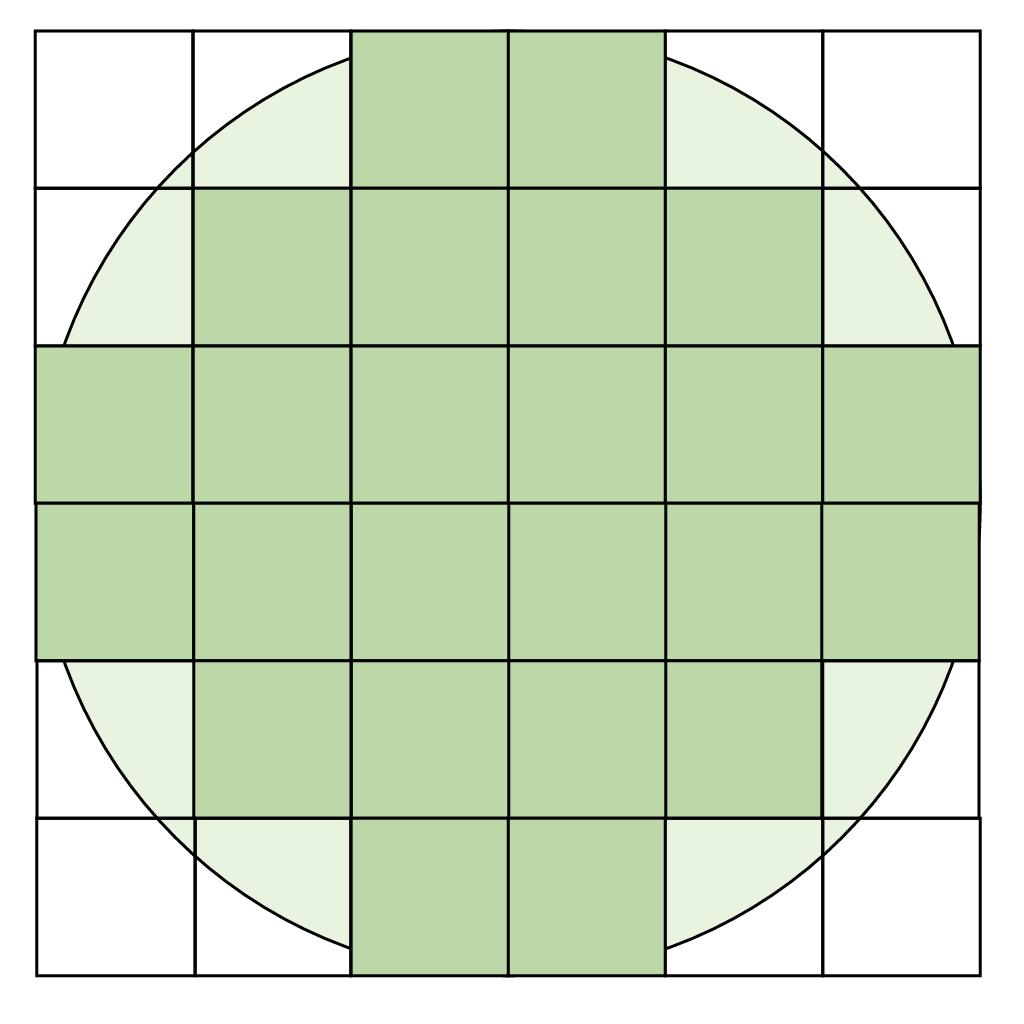
\includegraphics[scale=0.15]{figures/PixelCircleSquare.png}
	\caption{A circle in a possible pixel presentation. All small squares present pixels. The colored squares present the pixels, which are included in the pixel presentation of the circle.}
	\label{img:CircleSquarePixels}
\end{figure}

\begin{figure}
	\center
	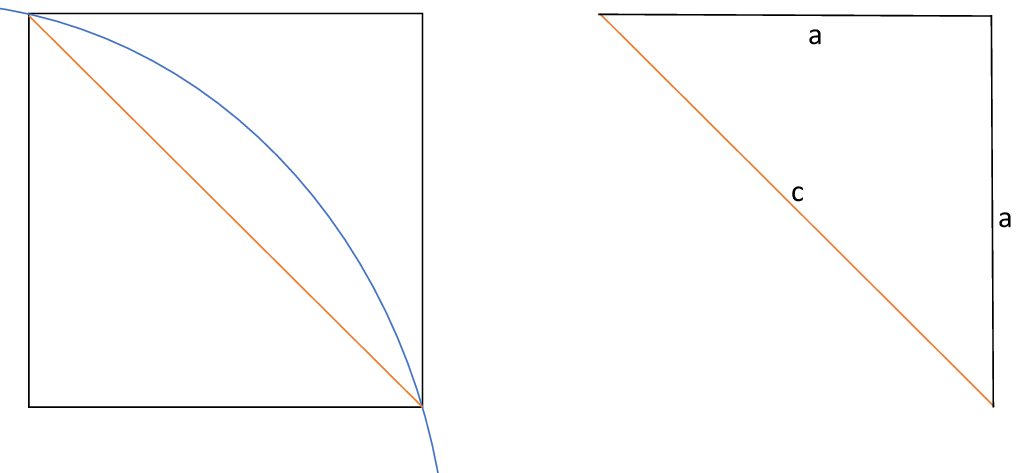
\includegraphics[scale=0.3]{figures/SurfaceApproximationSQRT2.png}
	\caption{The left part of the illustration displays a pixel at the surface, in which the circle goes through. The blue line represents the circle. As an approximation to the surface line a diagonal line in the square is drawn. With this diagonal line an isosceles, right ancular triangle appears and it is possible to calculate the additional surface of one pixel. This isosceles, right ancular triangle is displayed at the right side of this figure.}
	\label{img:ApproximationSQRT2}
\end{figure}

\begin{figure}
	\center
	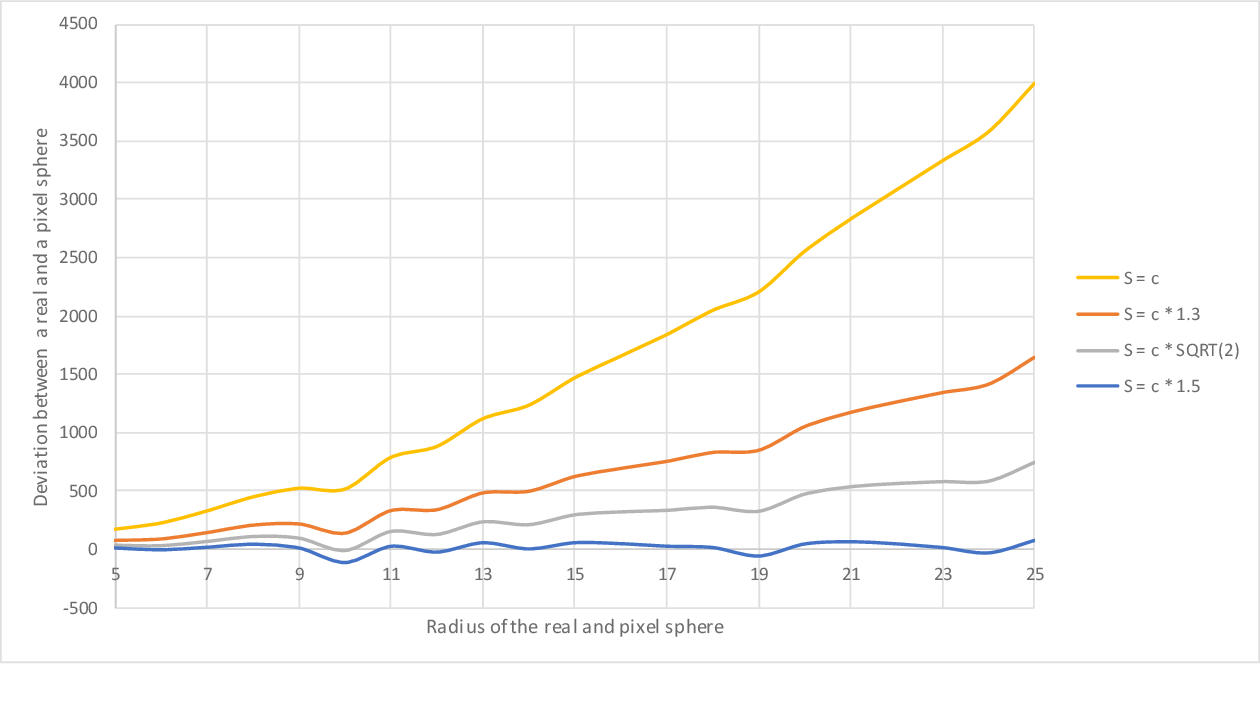
\includegraphics[scale=0.3]{figures/DeviationSphereToPixelSphere.png}
	\caption{Deviation between the surface of sphere of voxels and a real sphere. Each deviation is calculated with a different factor of the surface of the real sphere. $S$ refers to the surface of the sphere of voxels and $c$ refers to the surface of a real sphere. Thus, $c = 4 \cdot \pi \cdot r^{2}$. \newline
	At the x-axis the radius of the sphere and the sphere of voxels is displayed. At the y-axis the deviation between both surfaces is represented.}
	\label{img:DeviationSphere}
\end{figure}

In figure \ref{img:ApproximationSQRT2} the left square is considered as a pixel, it could be any pixel of the figure \ref{img:CircleSquarePixels} in which the circle goes through. Thus, the sides of the square are the same. The blue line represents the circle, in a way it could go through the pixel. An approximation is to insert a diagonal line. With this diagonal line an isosceles, right ancular triangle is created as it is displayed at the right side of figure \ref{img:ApproximationSQRT2}. \newline
The following formula provides a way to calculate the sides of the isosceles, right ancular triangle.
\begin{equation}\label{eq:IsoscelesRightAncularTriangle}
c^{2} = 2 \cdot a^{2}
\end{equation}
This formula can be used to calculate the side $a$, as it is displayed in the following equation.
\begin{equation}\label{eq:CornerSideAOfTriangle}
\begin{split}
a &= \sqrt{\dfrac{c^{2}}{2}} \\
a &= \dfrac{c \cdot \sqrt{2}}{2}
\end{split}
\end{equation}
Since the surface of a pixel has two corner sides, the equation to calculate the surface of a pixel sphere is
\begin{equation}\label{eq:PixelSurfaceCalculation}
\begin{split}
S &= 2a \\
S &= c \cdot \sqrt{2}
\end{split}
\end{equation}
This formula applies to all pixels, which are at the surface of the pixel sphere, $c$ is considered as the surface of the circle. Thus $c = \pi \cdot r^{2}$.

The calculated factor $\sqrt{2}$ was tested for a sphere surface. Because, this is an approximation to the surface of a pixel sphere, the tenth part beside this factor are also tested mathematically. As figure \ref{img:DeviationSphere} displays the  approximation with factor $\sqrt{2}$ still has some deviation. Almost no deviation between the surface of a sphere and a surface of a sphere of voxels is with a factor of $1.5$. Thus, this factor is applied for the calculation of the target surface. 

\section{Calculation of the volume and surface sites of a voxel sphere}
In order to calculate the voxel volume and the surface sites of a voxels sphere on our own, I created an algorithm for this problem. Otherwise for every measurement of the volume and surface of the sphere of voxels a new simulation in \ac{CC3D} had to be started. \newline
The algorithm requires the radius of the sphere, this radius has to be a whole number. For the tenths part between two whole numbers the result of the algorithm and \ac{CC3D} deviates.
Since a sphere and a cuboid are both symmetrical, it is possible to split both into 8 pieces. Doing so only one eighth of the of the cuboid has to be calculated in order to determine the volume and the surface of the sphere. \newline
To calculate which voxels are in the voxel sphere, the algorithm creates a x, z, y matrix. In the following calculations and decisions the center of each voxel is used. For every x,z voxel in the eighth of the cuboid the y constraint of the circle is calculated. Next, every voxel at the x,z coordinate is checked if the center of the voxel is within this constraint or not. Thus, every voxel at a x,z coordinate is checked if its center is within the sphere or not. This is repeated until every x,z coordinate of the eighth of the cuboid is calculated. Every time a voxel is within the sphere, it will be marked in the matrix.  \newline
To receive the volume of the voxel sphere all marked entries in the created matrix are count. Then, this result is mirrored for all three axis. Thus, the amount of marked voxels in the matrix is multiplied by 8, which equals to one multiply by 2 for each axis. Therefore $V=((Voxels \cdot 2) \cdot 2) \cdot 2$.
To receive the surface sites of the voxels at the surface, every marked entry is checked if the voxel at x+1, z+1 or the y+1 is either out of bounce, i.e. if it is outside the cuboid, or outside the sphere. Every of the three conditions is checked for every voxel within the surface. If one condition is true, the amount of surface sites is increased by 1. In the end the result, like the volume, has to multiplied by 8, in order to mirror the result for all three axis.



\chapter{Results}
This chapter presents the results of the bachelor thesis. Modifications which influence the structure of the program and the behavior of the simulation are presented at the beginning. Later the results of the desired cell as a sphere as well as the result of the created algorithm are revealed. In the last section evaluations of 3D simulations are shown.

\section{Structure of the program}
With the removement of unused methods and variables, the program becomes more readable and is easier to understand. These changes decrease the probability of errors and confusion during code analysis, i.e. studying of the code. By declaring abstract methods, the program becomes more structured. The program is easier to understand as well as it is easier to find errors, because identical methods are not written again in classes which inherit from each other. \newline
The changes described in section \ref{sec:LambdaMultipliers} and \ref{sec:AbstractMethods} modify the program in a way that it is more structured and understandable. This improves the time required for the code analysis, which is important for newcomers to the project, as well as to find errors.


\section{Improvements of the program}
During the bachelor thesis several adjustments in the program code were made. All these changes are important as they affect the simulation. These changes were tested by using the output command to see the required information at the command line. 
\subsection{Calculation of the amount of stem cells on the basal membrane}
With the changes presented in section \ref{sec:AmountStemCellsBasalMembrane} the program now has a calculation of the amount of stem cells on the basal membrane for two and three dimensions. The new calculation is correct for every simulation size in 2D and 3D. This is important as the program should be able to have a correct implementation for two as well as for three dimensions. An example for the initialization of a simulation is displayed in figure \ref{img:SimulationAtMCS0} at page \pageref{img:SimulationAtMCS0}.




\subsection{\ac{MCS} until the urination event}
The modifications of the calculation until the urination event was presented in section \ref{sec:calculationStpesUntilUrination}. Therefore, the urination now takes place every six hours instead of every twelve hours. This change is important for the simulation because with a urination every twelve hours the simulation is not as real as with the event every six hours. Moreover, in the paper \cite{Torelli2017} of the project it is stated that this event occurs every six hours. This change helps the simulation to not only be more realistic, it is also important that there are not too many cells in the simulation field. As a result of too many cells in the simulation field the simulation stops. Thus, the change increases the quality of a simulation and helps to prevent an overflow of cells.
\subsection{Target volume and target surface after mitosis}
The described modifications in section \ref{sec:TargetVolumeSurfaceAfterMitosis} affects the simulation in a way that after mitosis both cells are able to grow immediately. Without the modification the cell with a too small target volume and target surface would not grow several calculation steps. Therefore, the cell does not grow until the target volume becomes larger than the current volume. It is not possible that one of the two cells have a smaller target volume and surface than the current volume and surface, because the target volume of both created cells is now set dependent on the by \ac{CC3D} given volume of each cell. With this modification both cells, created during mitosis, are now able to grow immediately.
\subsection{Conversion between the physical unit and the voxel unit}
The modifications presented in section \ref{sec:ApproximationError} are crucial since now the calculation of volume constraints of each cell type is more precise. With this modification every conversion of \SI{}{\micro\metre} into pixels and voxels is now free of calculation errors. Since the result of the calculations of the volume constraints of the different cell types is used to determine when mitosis takes place it is important to have it without a calculation error. Simulations beside a voxel density of one have the correct volume constraints of the cells, because the result is converted only at the end. Moreover, this calculation is also used to calculate the growth per calculation step in the simulation, since the growth of a cell is calculated in the physical unit and then converted into pixels. This modification is important and affects the correctness of simulations, because the calculation of the volume constraints of the different cell types and the calculation of the growth of each cell each \ac{MCS} are two major parts of the simulation.\newline
\newpage
\begin{figure}[h]
	\center
	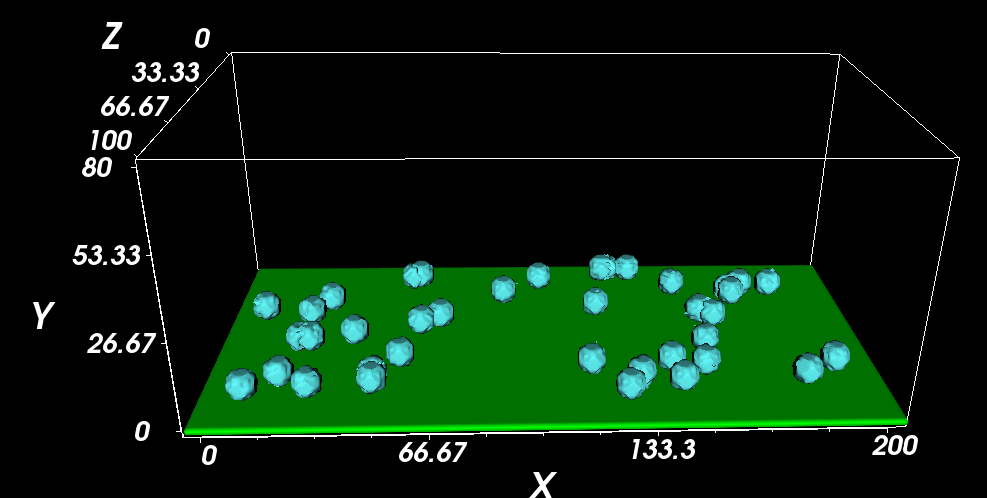
\includegraphics[scale=0.4]{figures/SimulationAtMCS0.png}
	\caption[Spread stem cells at the basal membrane at \ac{MCS} 0]{Spread stem cells at the basal membrane at \ac{MCS} 0. The box displays the simulation field, with a size of \SI{100}{\micro\metre} at the x-asis, \SI{80}{\micro\metre} at the y-axis and \SI{100}{\micro\metre} at the z-axis. In the simulation the green bottom displays the basal membrane and at the basal membrane the stem cells are spread. The amount of these stem cells is calculated as explained in section \ref{sec:AmountStemCellsBasalMembrane}.}
	\label{img:SimulationAtMCS0}
\end{figure}




\section{Draw sphere cells}
With the new method presented in section \ref{sec:DrawSphereCells} the program is now able to draw a sphere cell, as it is displayed in figure \ref{img:DrawnSphereCells}. \newline
Since voxels are used in the 3D simulation to draw a sphere cell it is not possible to draw a perfectly round sphere. This problem is displayed with an circle and a square in picture \ref{img:CircleSquarePixels} at page \pageref{img:CircleSquarePixels}, since the circle and square are the 2D presentation of a sphere and a cuboid. The drawn cells are as spherish as possible in the simulation with the use of voxels. \newline
Figure \ref{img:DrawnSphereCells} displays independently drawn cells with different radius of \SI{5}{\micro\metre} and up to \SI{23}{\micro\metre}. The cells in the first two rows show that there are a lot of edges in the sphere. As the radius increases, the sphere shape of the cell gets more detailed as it is displayed in the last two rows. With the increase of the radius the deviation of the surface increases as well, as it is shown in figure \ref{img:DeviationSphere} at page \pageref{img:DeviationSphere}. This might be a result as the surface of a sphere and a cuboid, with the diameter $2 \cdot r$, deviates more as $r$ increases.


\begin{figure}[!]
	\begin{center}
	\subfloat[]{
		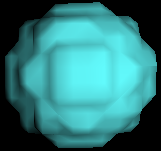
\includegraphics[scale=0.75]{figures/VoxelSphere/Radius5-0.png}
	}
	\subfloat[]{
		\hspace{1.5cm}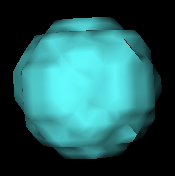
\includegraphics[scale=0.755]{figures/VoxelSphere/Radius5-1.png}
	}
	\end{center}
	\begin{center}
	\subfloat[]{
		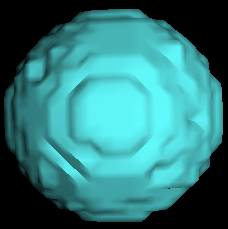
\includegraphics[scale=0.53]{figures/VoxelSphere/Radius9-0.png}
	}
	\subfloat[]{
		\hspace{1.5cm}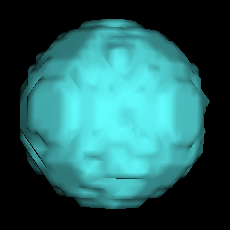
\includegraphics[scale=0.54]{figures/VoxelSphere/Radius9-1.png}
	}
	\end{center}
	
		\begin{center}
	\subfloat[]{
		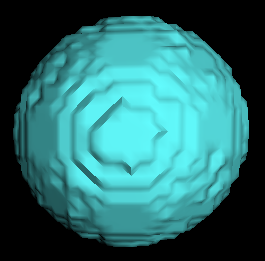
\includegraphics[scale=0.455]{figures/VoxelSphere/Radius14-0.png}
	}
	\subfloat[]{
		\hspace{1.5cm}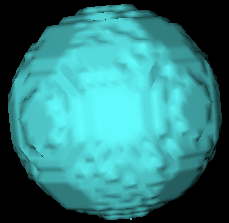
\includegraphics[scale=0.545]{figures/VoxelSphere/Radius14-1.png}
	}
	\end{center}
	\begin{center}
	\subfloat[]{
%		\hspace{0.1cm}
		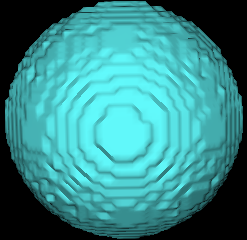
\includegraphics[scale=0.505]{figures/VoxelSphere/Radius23-0.png}
	}
	\subfloat[]{
		\hspace{1.5cm}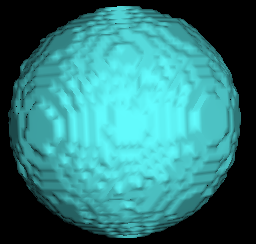
\includegraphics[scale=0.49]{figures/VoxelSphere/Radius23-1.png}
	}
	\end{center}
	
	
	\caption[Drawn sphere cells]{\label{img:DrawnSphereCells}A single cell drawn into the simulation field. The radius of the cell in the first row is \SI{5}{\micro\metre}, in the second row a cell with a diameter of \SI{9}{\micro\metre} is displayed, in the third row a diameter of \SI{14}{\micro\metre} was used and in the last row the cell has a diameter of \SI{23}{\micro\metre}. The pictures in the left column are with the front view, whereas the
pictures at the right column have a view angle of around 45 degrees.}
\end{figure}



\section{Calculate the voxel volume and surface sites of a sphere cell}
The created algorithm, which is described in section \ref{sec:CreatedAlgorithm} it is able to calculate, out of a given radius, the volume of a sphere cell created with cuboids in voxel, as well as it is able to count the surface sites of the cell. Moreover, it is also possible to calculate the physical volume and surface of a sphere with a given radius. With this algorithm it is possible to calculate the volume and surface of a sphere cell and get the same result as \ac{CC3D} calculates. \newline
The algorithm is useful but also has its weaknesses. For a voxel density beside one the results between the created algorithm and \ac{CC3D} deviate. The results differ also if the radius is not a whole number. There are no insights how \ac{CC3D} calculates the volume and surface of a drawn sphere cell. Moreover, for the tenths part of five to nine of the radius, for every radius between $.5$ until $.9$, it is possible to create the cube with a radius which is either rounded up or down. This means for a radius of $3.7$ it is possible to use either six or eight voxels to create the cuboid. Seven voxels are not possible because then the sphere would lose its symmetry. \newline
The algorithm helps to calculate the volume of a sphere cell, out of voxels, as well as to count the surface sites. It is able to be executed without a start of a simulation. Thus, there is no need to adjust the coding of the project and to wait until the simulation started to receive the volume and surface values of a sphere cell.


\section{Growth of sphere cells}\label{sec:GrowSphereCells}
In section \ref{sec:GrowSphereCell} the factor for the calculation of the surface of the cell was evidenced best to be $1.5$ for a voxel density of one. With this factor it should be possible to let the sphere cell grow as a sphere. To test the growth of the cell, one single cell was placed in the simulation field. As the cell grew during the simulation the volume and surface values were read out of the command line and compared to the documented values of a drawn cell. \newline
To let a cell grow as a sphere does not work. Even the volume and surface values, calculated by \ac{CC3D}, and the target volume and target surface values, calculated by the program, meet the values of sphere cells with a small deviation of a maximum deviation up to 50 voxels. \newline
In figure \ref{img:GrowthSphereCellRadius5} and \ref{img:GrowthSphereCellRadius9} examples of the growth of two stem cells with a different radius are displayed. It is observable that these cells are not able to keep the shape with which they were depicted.


\begin{figure}[H]
	\begin{center}
	\subfloat[]{
		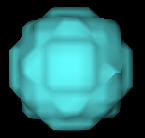
\includegraphics[scale=0.85]{figures/GrowthSphereCell/Radius5/Radius5-MCS0.png}
	}
	\subfloat[]{
		\hspace{1.5cm}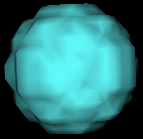
\includegraphics[scale=0.842]{figures/GrowthSphereCell/Radius5/Radius5-MCS0-1.png}
	}
	\end{center}
	\begin{center}
	\subfloat[]{
		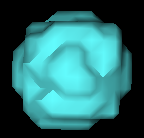
\includegraphics[scale=0.86]{figures/GrowthSphereCell/Radius5/Radius5-MCS50.png}
	}
	\subfloat[]{
		\hspace{1.5cm}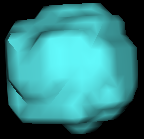
\includegraphics[scale=0.855]{figures/GrowthSphereCell/Radius5/Radius5-MCS50-1.png}
	}
	\end{center}
	\begin{center}
	\subfloat[]{
		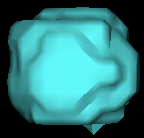
\includegraphics[scale=0.845]{figures/GrowthSphereCell/Radius5/Radius5-MCS250.png}
	}
	\subfloat[]{
		\hspace{1.53cm}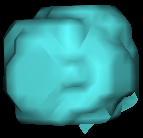
\includegraphics[scale=0.845]{figures/GrowthSphereCell/Radius5/Radius5-MCS250-1.png}
	}
	\end{center}
	\caption[Growth of a sphere cell with a radius of 5]{\label{img:GrowthSphereCellRadius5}A sphere cell, with a radius of \SI{5}{\micro\metre} and a voxel density of one, as it grows. Images (a), (c) and (e) show the front view of the cell and figures (b), (d) and(f) have around a 45 degrees angle of the front. Figure (a) and (b) are at \ac{MCS} 0, images (c) and (d) at calculation step 50 and figures (e) and (f) present \ac{MCS} 250.}
\end{figure}

\begin{figure}[H]
	\begin{center}
	\subfloat[]{
		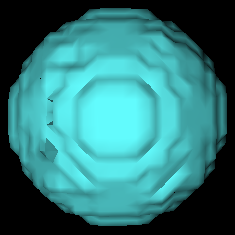
\includegraphics[scale=0.5]{figures/GrowthSphereCell/Radius9/Radius9-MCS0.png}
	}
	\subfloat[]{
		\hspace{1.5cm}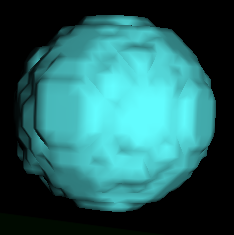
\includegraphics[scale=0.5]{figures/GrowthSphereCell/Radius9/Radius9-MCS0-1.png}
	}
	\end{center}
	\begin{center}
	\subfloat[]{
		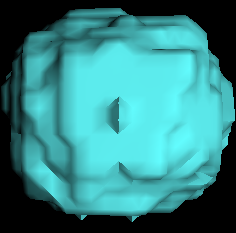
\includegraphics[scale=0.5]{figures/GrowthSphereCell/Radius9/Radius9-MCS250.png}
	}
	\subfloat[]{
		\hspace{1.5cm}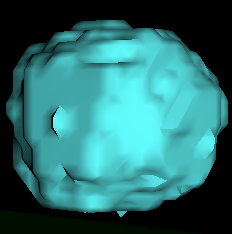
\includegraphics[scale=0.498]{figures/GrowthSphereCell/Radius9/Radius9-MCS250-1.png}
	}
	\end{center}
	\begin{center}
	\subfloat[]{
		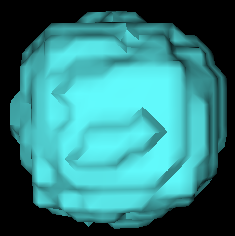
\includegraphics[scale=0.5]{figures/GrowthSphereCell/Radius9/Radius9-MCS750.png}
	}
	\subfloat[]{
		\hspace{1.5cm}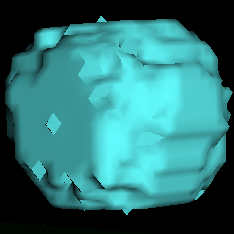
\includegraphics[scale=0.5]{figures/GrowthSphereCell/Radius9/Radius9-MCS750-1.png}
	}
	\end{center}
	\caption[Growth of a sphere cell with a radius of 9]{\label{img:GrowthSphereCellRadius9}A sphere cell, with a radius of \SI{9}{\micro\metre} and a voxel density of one, as it grows. Images (a), (c) and (e) show the front view of the cell and figures (b), (d) and (f) have an approximately 45 degrees angle of the front. Figures (a) and (b) are at \ac{MCS} 0, figures (c) and (d) at calculation step 250 and figures (e) and (f) present \ac{MCS} 750.}
\end{figure}

\newpage

\section{Adhesion matrix}
The new adhesion matrix is different from the one which was used until this thesis. Based on the observations of section \ref{sec:AdhesionMatrix} the new adhesion matrix was created. The matrix is displayed in table \ref{tbl:NewAdhesion}. The values were chosen in a way that cells of one layer stick to each other and try to increase the area where the cells touch. The adhesion for cells at one layer was observed not to be too high in order that the cells do not infiltrate each other. An example therefor is displayed in figure \ref{img:InfiltratingCells}. If cells infiltrate each other it is a sign of too high adhesion energy. For the adhesion between cells of different layers in the urothelium the values were chosen in a way that the cells connect with each other but that they grow independently. It is important that the cells of different layers do not connect too strong to each other, otherwise the different layers in the urothelium might be mixed. 

\begin{figure}[H]
	\center
	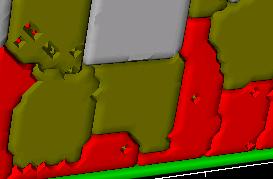
\includegraphics[scale=1.2]{figures/TooHighAdhesion1.png}
	\caption[Different cells try to infiltrate each other]{Different cells try to infiltrate each other as a reason of too high adhesion values between the cells. The different points at the surface of a cell are an indicator that a surrounding cell tries to infiltrate the cell at which the points occur.}
	\label{img:InfiltratingCells}
\end{figure}


\begin{table}[ht]
\centering
\caption[New adhesion values for the different cell types]{New adhesion values for the adhesion between the different cell types. M, the medium cell type, is a by \ac{CC3D} specific cell type for the simulation.\newline}
\renewcommand{\arraystretch}{1.5}
	\begin{tabular}{|c|c||c|c|c|c|c|c|}
	\hline
		\multicolumn{2}{|c||}{Types} & M & BM & S & B & I & U \\
		\hline
		\hline
		
		Medium & M & 0 & 14 & 14 & 14 & 14 & 14 \\
		\hline
		Basal membrane & BM & & -1 & 2 & 3 & 30 & 30 \\
		\hline
		Stem cell & S & & & 12 & 15 & 25 & 25 \\
		\hline
		Basal cell & B & & & & 12 & 25 & 25 \\
		\hline
		Intermediate cell & I & & & & & 6 & 25 \\
		\hline
		Umbrella cell & U & & & & & & 2
\tabularnewline
\hline 
	\end{tabular}
	\label{tbl:NewAdhesion}
\end{table}

\newpage

\section{Simulation result}
To test this bachelor thesis some 3D simulations were made. It is not possible to have an in depth analysis of several simulations, because a 3D simulation over a timespan of 700 days with a simulation field of \SI{200}{\micro\metre} at the x-axis, \SI{80}{\micro\metre} at the y-axis and \SI{100}{\micro\metre} at the z-axis and with a voxel density of one took 14 days to complete. Because of this immense time effort, a brief analysis of one simulation run of the model SPA/PCDB/PCDI is provided. In the next chapter analyses of short simulations are compared briefly to the completed simulation presented in this chapter. \newline
Figure \ref{img:720daysScreenshotSPA/BCPD/IPCD} at page \pageref{img:720daysScreenshotSPA/BCPD/IPCD} displays screenshots at the front and at the back of the simulation field. These screenshots are taken after the simulation was finished. It is visible that the arrangement of the cell layers is not perfect, because some umbrella cells are on top of the basal cells. Moreover, at one point an intermediate cell is surrounded by umbrella cells, therefore it is at a wrong layer in the urothelium. \newline
In figure \ref{img:Fa_Fv_SPA/BCPD/IPCD} the result of the fitness functions of section \ref{sec:fitnessFunctions} is provided. The arrangement fitness function displays an almost perfect result of an urothelium, whereas the volume and the total fitness functions display not much reality in the simulation. The 2D simulation of this model had an overall fitness value of almost 90\% by 49 simulation runs. In the 3D simulation the overall fitness values is lower. Why this decrease happen and a further analysis of this simulation and of other simulations is discussed in the next chapter in section \ref{sec:SimulationResults}.

%With the results of the simulations a first insight of the 3D simulation is given. To receive a complete and in detail analysis of the models in three dimensions several simulations of the different models has to be done.
\begin{figure}[ht]
\begin{center}
\begin{tikzpicture} 
\begin{axis}[
xlabel=$t$ in days,
ylabel=Fitness,
grid=major,
xmin=0,xmax=700,ymin=0,ymax=1,
width=10cm,height=10cm,
legend entries={$f_A$, $f_V$, $f_{T}$},
legend style={at={(0.02,0.02)},anchor=south west}
]
\addplot[
color=blue,
mark repeat=0.5, mark phase=0
] table[x=time,y=FitnessTotal] {figures/SpaPcdbPcdiIn/FitnessPlot.dat}; 
\addplot[
color=gray,
mark repeat=0.5, mark phase=0
] table[x=time,y=FitnessArrangement] {figures/SpaPcdbPcdiIn/FitnessArrangement.dat}; 
\addplot[
color=darkgreen,
mark repeat=0.5, mark phase=0
] table[x=time,y=FitnessVolume] {figures/SpaPcdbPcdiIn/FitnessVolume.dat}; 
\end{axis}
\end{tikzpicture}
\caption[Analysis of a simulation of the model SPA/BCPD/IPCD]{\label{img:Fa_Fv_SPA/BCPD/IPCD}Analysis of a simulation of the model SPA/BCPD/IPCD. The simulation covered 700 days, 350000 \ac{MCS}. The analysis covers the arrangement, $f_{A}$, the volume fitness function, $f_{V}$ and the overall fitness function $f_{T}$ of section \ref{sec:fitnessFunctions}. At the figure the 'Fitness' values represent the reality of this model, where 0 refers to no reality and 1 presents a perfect realistic simulated urothelium.}

\end{center}
\end{figure}

\begin{figure}[ht]
\begin{center}
\subfloat[]{
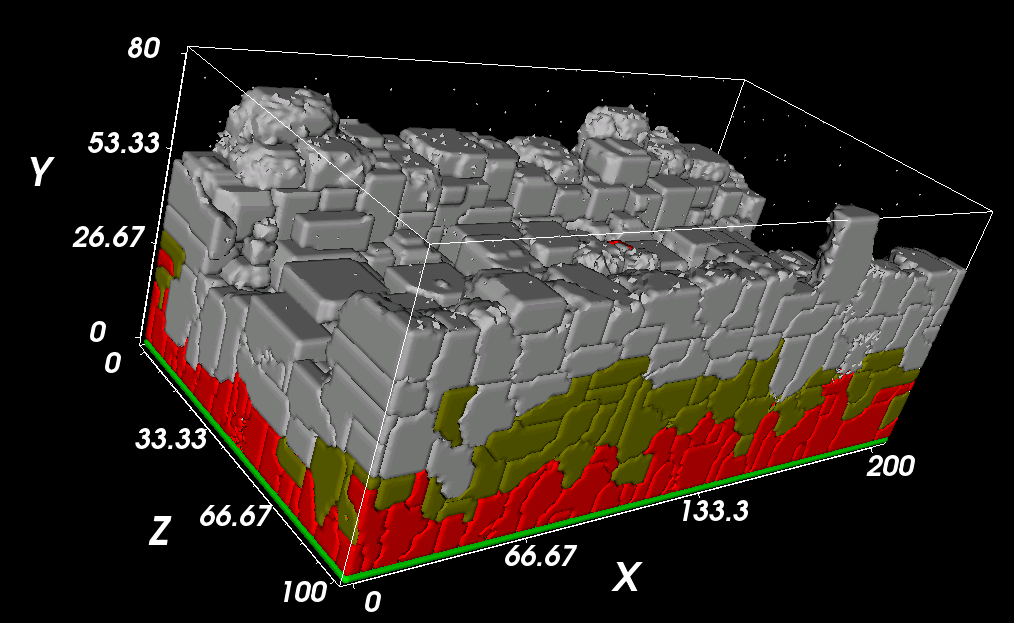
\includegraphics[width=12cm]{figures/SpaPcdbPcdiIn/MCS350000.png}
}
\end{center}
\begin{center}
\subfloat[]{
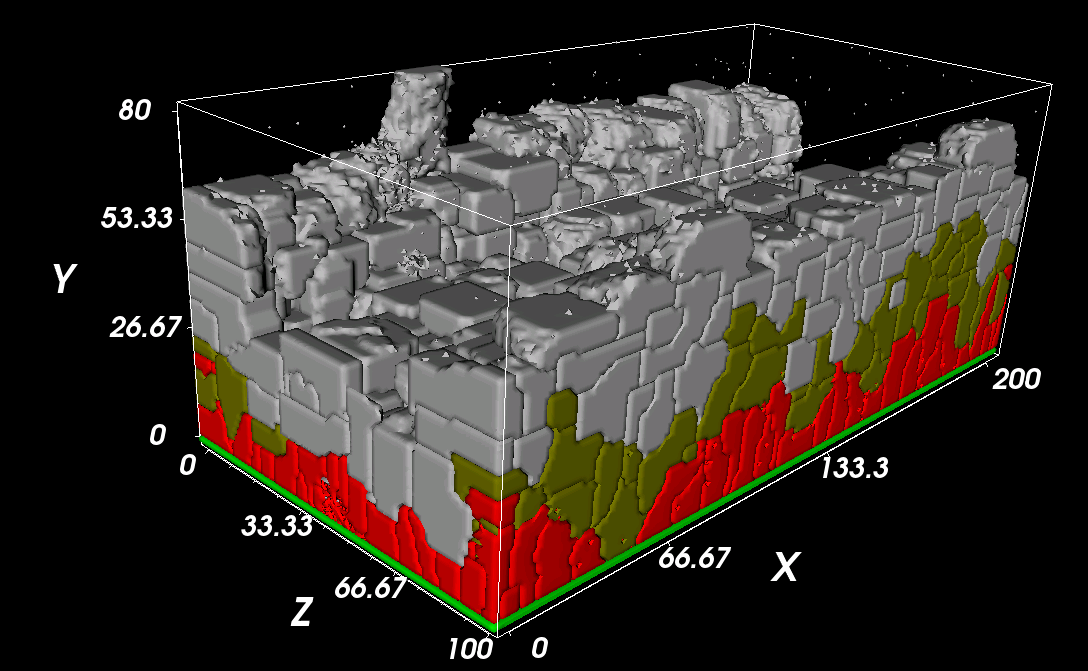
\includegraphics[width=12cm]{figures/SpaPcdbPcdiIn/MCS350000-1.png}
}
\end{center}
\caption[Simulated urothel with the model SPA/PCDB/PCDI at day 700]{\label{img:720daysScreenshotSPA/BCPD/IPCD}Screenshots at the end of a simulation of the model SPA/PCDB/PCDI, which lasted 700 days. Screenshot (a) is taken of the front view, whereas screenshot (b) is taken of the back of the urothelium.}

\end{figure}




\chapter{Conclusion}
Final words

\section{Draw Sphere Cells}
It is also possible to use only the effective energy

\section{lambda values}
This was the only way to do it

\section{Approximation Errors}
Find a more elegant way to do it
% ------------------------------------------------------------------

\label{lastpage}

% Neue Seite
\cleardoublepage

% Backmatter mit normalem Zeilenabstand setzen
\singlespacing

% Römische Ziffern für die "Back-Matter", fortlaufend mit "Front-Matter"
\pagenumbering{roman}
\setcounter{page}{\value{frontmatterpage}}

% Abkürzungsverzeichnis
\addchap{\hsmaabbreviations}
% Die längste Abkürzung kann in die eckigen Klammern
% bei \begin{acronym} geschrieben, um einen häßlichen
% Umbruch zu verhindern
\begin{acronym}[IEEE]
\acro{ABK}{Abkürzung}
\acro{ACM}{Association of Computing Machinery}
\acro{PDF}{Portable Document Format}
\acro{IEEE}{Institute of Electrical and Electronics Engineers}
\acro{ISO}{International Organization for Standardization}



\acro{GGH}{Glazier-Graner-Hogeweg}
\acro{CC3D}{CompuCell3D}
\acro{ECM}{Extended Cellular Matrix}
\acro{MCS}{Monte Carlo Step}
\acro{CPM}{Cellular Potts Model}
\acro{EPM}{Extended Potts Model}
\acro{OOP}{Object Oriented Programming}
\acro{CPU}{Central Processing Unit}
\acro{RW}{Random Walker}
\acro{VM}{Virtual Machine}
\end{acronym}


% Tabellenverzeichnis erzeugen
\cleardoublepage
\phantomsection
\addcontentsline{toc}{chapter}{\hsmalistoftables}
\listoftables

% Abbildungsverzeichnis erzeugen
\cleardoublepage
\phantomsection
\addcontentsline{toc}{chapter}{\hsmalistoffigures}
\listoffigures

% Listingverzeichnis erzeugen
\cleardoublepage
\phantomsection
\addcontentsline{toc}{chapter}{\hsmalistings}
\lstlistoflistings

% Literaturverzeichnis erzeugen
\begin{flushleft}
\printbibliography
\end{flushleft}

% Index ausgeben. Wenn Sie keinen Index haben, entfernen Sie einfach
% diesen Teil.
\cleardoublepage
\phantomsection
\addcontentsline{toc}{chapter}{\hsmaindex}
\printindex

% Anhang. Wenn Sie keinen Anhang haben, entfernen Sie einfach
% diesen Teil.
\appendix
\chapter{Erster Anhang}

Hier ein Beispiel für einen Anhang. Der Anhang kann genauso in Kapitel und Unterkapitel unterteilt werden, wie die anderen Teile der Arbeit auch.

\chapter{Zweiter Anhang}

Hier noch ein Beispiel für einen Anhang.


\end{document}
